\documentclass[hyperref={bookmarks=false},aspectratio=169]{beamer}
\usepackage{hyperref,ragged2e,amsmath,amssymb,url,bm}
\usepackage{graphicx,booktabs,array}
\usepackage{tikz}
\usetikzlibrary{arrows.meta,positioning,calc,shapes.geometric,decorations.pathreplacing,matrix}
\graphicspath{{crops/}}
\usetheme{Goettingen}
% --- Paleta de la serie Festividades santas: tierra roja, café rojizo, mostaza y papiro ---
\definecolor{tierraroja}{RGB}{122,40,18}
\definecolor{caferojizo}{RGB}{58,18,8}
\definecolor{mostaza}{RGB}{214,160,58}
\definecolor{papiro}{RGB}{243,228,192}
\definecolor{sepia}{RGB}{98,66,44}
\definecolor{oliva}{RGB}{92,98,48}
\setbeamercolor{structure}{fg=tierraroja}
\setbeamertemplate{sidebar canvas right}[vertical shading][top=tierraroja!92!black,bottom=caferojizo]
\setbeamercolor{title in sidebar}{fg=mostaza}
\setbeamercolor{author in sidebar}{fg=papiro}
\setbeamercolor{section in sidebar}{fg=papiro}
\setbeamercolor{section in sidebar shaded}{fg=mostaza!55!papiro!75!tierraroja}
\setbeamercolor{subsection in sidebar}{fg=papiro}
\setbeamercolor{subsection in sidebar shaded}{fg=mostaza!55!papiro!75!tierraroja}
\let\raggedright\justifying
\setlength{\RaggedRightRightskip}{0pt plus 1fil}
\setbeamertemplate{background canvas}{
\includegraphics[width=\paperwidth,height=\paperheight]{papiro.jpg}}
\setbeamercolor{normal text}{fg=caferojizo!90!black}
\setbeamercolor{frametitle}{fg=tierraroja}
\setbeamerfont{frametitle}{series=\bfseries}
\setbeamertemplate{section in toc shaded}{\leavevmode{\color{sepia!85!black}\inserttocsection}\par}
\setbeamercolor{title}{fg=tierraroja}
\setbeamercolor{subtitle}{fg=sepia}
\setbeamercolor{item projected}{bg=tierraroja,fg=papiro}
\setbeamertemplate{itemize item}{\small\textcolor{mostaza!80!tierraroja}{$\blacktriangleright$}}
\setbeamertemplate{navigation symbols}{}
% --- Español + hebreo + griego (XeLaTeX) con fuentes empaquetadas en fonts/ ---
\usepackage[bidi=default]{babel}
\babelprovide[import,main]{spanish}
\babelprovide[import]{hebrew}
\babelprovide[import]{ancientgreek}
\babelfont[hebrew]{sf}[Path=fonts/, BoldFont=NotoHebrewSans-700.ttf]{NotoHebrewSans-400.ttf}
\babelfont[hebrew]{rm}[Path=fonts/, BoldFont=NotoHebrewSans-700.ttf]{NotoHebrewSans-400.ttf}
\babelfont[ancientgreek]{sf}[Path=fonts/]{GFSPorson.otf}
\babelfont[ancientgreek]{rm}[Path=fonts/]{GFSPorson.otf}
\newcommand{\heb}[1]{\mbox{\foreignlanguage{hebrew}{#1}}}
\newcommand{\grc}[1]{\foreignlanguage{ancientgreek}{#1}}
\newcommand{\SENOR}{S{\fontsize{0.78em}{1em}\selectfont EÑOR}}
% --- Citas, imágenes, referencias ---
\usepackage[most]{tcolorbox}
\newtcolorbox{cita}[1][]{enhanced, colback=papiro, opacityback=0.80, colframe=tierraroja!85!mostaza,
  boxrule=0pt, leftrule=2.5pt, arc=0pt, left=6pt, right=6pt, top=4pt, bottom=4pt,
  before skip=4pt, after skip=6pt, fontupper=\small\itshape, #1}
\newcommand{\fuente}[1]{\par\hfill{\upshape\bfseries\footnotesize\textcolor{tierraroja}{#1}}}
\newcommand{\imagen}[3][0.80]{%
  \centering\includegraphics[height=#1\textheight,width=\linewidth,keepaspectratio]{#2}\par\vspace{2pt}
  {\fontsize{5}{6}\selectfont\color{sepia}{\raggedleft\textit{Nota.} #3\par}}}
\makeatletter
\newcommand{\fotolado}[2]{%
  \begin{tikzpicture}[remember picture,overlay]
    \node[anchor=north east,inner sep=0pt] (foto) at ([xshift=-\beamer@sidebarwidth]current page.north east)
      {\includegraphics[height=\paperheight]{#1}};
    \node[anchor=south east,inner sep=2pt,text=papiro,fill=caferojizo,fill opacity=0.55,text opacity=1,
      font=\fontsize{4.5}{5.5}\selectfont,align=right,text width=4.2cm] at ([xshift=-3pt,yshift=3pt]foto.south east)
      {\textit{Nota.} #2};
  \end{tikzpicture}}
\makeatother
\newcommand{\refapa}[1]{\par{\RaggedRight\hangindent=1.2em\hangafter=1\noindent #1\par}\vspace{3pt}}
\usepackage{xurl}\urlstyle{same}
\newcommand{\destacar}[1]{\textbf{\textcolor{tierraroja}{#1}}}
\newcommand{\precision}[1]{{\footnotesize\color{sepia}\textbf{Precisión:} #1}}
\newcolumntype{L}[1]{>{\RaggedRight\arraybackslash}p{#1}}
\tikzset{caja/.style={draw=tierraroja,line width=0.8pt,fill=papiro,fill opacity=0.90,text opacity=1,rounded corners=3pt,inner sep=5pt,font=\scriptsize}}
\title[Shavuot]{\bfseries{Shavuot: la fiesta de las Semanas (Pentecostés)}}
\subtitle{``Hasta el día siguiente del séptimo día de reposo contaréis cincuenta días'' (Lv 23:16)}
\author{}\institute{}\date{}
\titlegraphic{
\includegraphics[width=0.80\linewidth,height=0.34\textheight,keepaspectratio]{portada.jpg}\\[-1pt]
  {\fontsize{5}{6}\selectfont\color{sepia}\textit{Nota.} Elaboración propia: Lv 23:16a en texto hebreo consonántico (BHS).}}
\begin{document}
\frame{\titlepage}

\begin{frame}\frametitle{Contenidos}\tableofcontents\end{frame}

% ------------------------------------------------------------------
\section{Introducción}

\begin{frame}{Una fiesta a la que se llega contando}
\begin{columns}[c,onlytextwidth]
\begin{column}{0.52\textwidth}\small
Pésaj, Matsot, Teruá, Kipur y Sukkot tienen día y mes. Shavuot carece de ellos: el texto manda \destacar{``contaréis''}, y Israel llega a la fiesta tras cuarenta y nueve días, desde la primera gavilla de cebada hasta el trigo maduro.\par\medskip
\begin{tcolorbox}[colback=papiro,colframe=tierraroja,boxrule=1pt,arc=3pt,left=4pt,right=4pt]
\RaggedRight\small\textbf{Tesis de la serie:} la fiesta de la siega es el \destacar{memorial} del Sinaí y de la entrega de la Ley, y la \destacar{figura} del derramamiento del Espíritu (Hch 2).
\end{tcolorbox}
\end{column}
\begin{column}{0.45\textwidth}\small
\begin{itemize}
\item ¿Qué se cuenta? Las siete semanas de la siega (Dt 16:9).
\item ¿Hacia qué? Una \destacar{ofrenda nueva}: dos panes leudados (Lv 23:16--17).
\item ¿Qué ocurrió ese día? ``Cuando llegó el día de Pentecostés\ldots'' (Hch 2:1).
\end{itemize}\medskip
\precision{el estudio separa lo explícito del texto de lo que es tradición o tipología.}
\end{column}
\end{columns}
\end{frame}

\begin{frame}{El ciclo de Levítico 23}
\centering
\resizebox{\linewidth}{!}{%
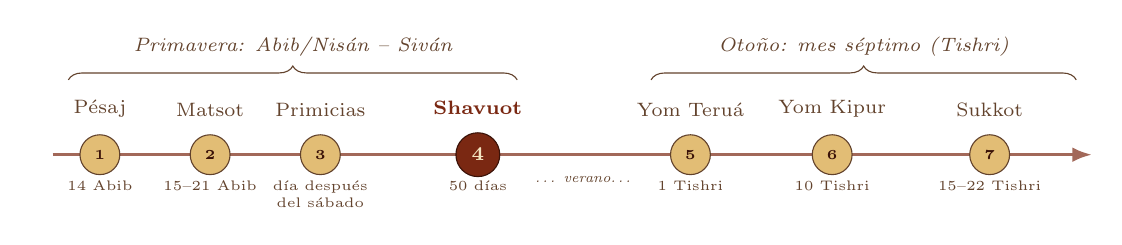
\begin{tikzpicture}[x=1cm,y=1cm,font=\scriptsize]
 \def\fiestaactual{4}
 \draw[line width=1.2pt,tierraroja!70,-{Latex[length=2.5mm]}] (0,0) -- (13.2,0);
 \draw[decorate,decoration={brace,amplitude=5pt},sepia] (0.2,0.95) -- (5.9,0.95) node[midway,above=5pt,font=\scriptsize\itshape]{Primavera: Abib/Nisán -- Siván};
 \draw[decorate,decoration={brace,amplitude=5pt},sepia] (7.6,0.95) -- (13.0,0.95) node[midway,above=5pt,font=\scriptsize\itshape]{Otoño: mes séptimo (Tishri)};
 \foreach \n/\x/\t/\d in {1/0.6/Pésaj/{14 Abib},2/2.0/Matsot/{15--21 Abib},3/3.4/Primicias/{día después del sábado},4/5.4/Shavuot/{50 días},5/8.1/Yom Teruá/{1 Tishri},6/9.9/Yom Kipur/{10 Tishri},7/11.9/Sukkot/{15--22 Tishri}}{
   \ifnum\n=\fiestaactual
     \node[circle,fill=tierraroja,draw=caferojizo,minimum size=5.5mm,text=papiro,font=\scriptsize\bfseries] at (\x,0) {\n};
     \node[above=3pt,font=\scriptsize\bfseries,text=tierraroja] at (\x,0.28) {\t};
   \else
     \node[circle,fill=mostaza!70,draw=sepia,minimum size=4.5mm,text=caferojizo,font=\tiny\bfseries] at (\x,0) {\n};
     \node[above=3pt,text=sepia] at (\x,0.25) {\t};
   \fi
   \node[below=6pt,text width=1.6cm,align=center,font=\tiny,text=sepia] at (\x,0) {\d};}
 \node[font=\tiny\itshape,text=sepia] at (6.75,-0.32) {\ldots\ verano\ldots};
\end{tikzpicture}}\par\medskip
\small\RaggedRight Shavuot \destacar{cierra la primavera}. Pésaj, Matsot y la gavilla caben en una semana; Shavuot viene siete semanas después, unida a ellas por la cuenta. Para la serie, la primavera mira a lo ya cumplido: la cruz, la salida del pecado, la resurrección y el don del Espíritu.
\end{frame}

% ------------------------------------------------------------------
\section{El texto}

\begin{frame}{Texto ancla: Lv 23:15--17}
\fotolado{panel_levitico23.jpg}{Elaboración propia: Lv 23:16 en texto hebreo consonántico (BHS).}
\begin{columns}[c,onlytextwidth]
\begin{column}{0.57\textwidth}
\begin{cita}Y contaréis desde el día que sigue al día de reposo, desde el día en que ofrecisteis la gavilla de la ofrenda mecida; siete semanas cumplidas serán. Hasta el día siguiente del séptimo día de reposo contaréis cincuenta días; entonces ofreceréis el nuevo grano a \SENOR.\fuente{(Lv 23:15--16, RVR1960)}\end{cita}
\small Tres verbos: \destacar{contar} (\heb{וּסְפַרְתֶּם}), \destacar{traer} (\heb{תָּבִיאוּ}), \destacar{ofrecer} (\heb{וְהִקְרַבְתֶּם}). La ofrenda es \heb{מִנְחָה חֲדָשָׁה} (\emph{minjá jadashá}), la primera del grano del año.
\end{column}
\begin{column}{0.41\textwidth}\end{column}
\end{columns}
\end{frame}

\begin{frame}{Dos panes y el borde del campo}
\begin{columns}[t,onlytextwidth]
\begin{column}{0.50\textwidth}
\centering\heb{חָמֵץ תֵּאָפֶינָה בִּכּוּרִים לַיהוָה}\par
\begin{cita}De vuestras habitaciones traeréis dos panes para ofrenda mecida\ldots{} de flor de harina, cocidos con levadura, como primicias para \SENOR.\fuente{(Lv 23:17)}\end{cita}
\scriptsize\RaggedRight No hay otros iguales en el calendario: vienen \destacar{de las casas}, son \destacar{dos}, de \destacar{trigo} y \destacar{leudados} (``cocidos con levadura'', \emph{jamets te'afena}), con la palabra que Matsot prohíbe (Éx 12:15).
\end{column}
\begin{column}{0.48\textwidth}
\begin{cita}Cuando segareis la mies de vuestra tierra, no segaréis hasta el último rincón de ella, ni espigarás tu siega; para el pobre y para el extranjero la dejarás. Yo \SENOR{} vuestro Dios.\fuente{(Lv 23:22)}\end{cita}
\scriptsize\RaggedRight La ley de la fiesta acaba en el \destacar{borde del campo}: \heb{פֵּאָה} (\emph{peá}, rincón) y \heb{לֶקֶט} (\emph{léqet}, espigueo) pertenecen al pobre (\heb{עָנִי}) y al extranjero (\heb{גֵּר}). Repite Lv 19:9--10.
\end{column}
\end{columns}
\end{frame}

\begin{frame}{Tabla sinóptica}
\scriptsize\renewcommand{\arraystretch}{1.12}
\begin{tabular}{@{}L{1.9cm}L{3.0cm}L{6.9cm}@{}}
\toprule
\textbf{Texto} & \textbf{Nombre} & \textbf{Lo que añade} \\ \midrule
Éx 23:16 & \heb{חַג הַקָּצִיר} \emph{jag haqatsir} & ``fiesta de la siega''; una de las tres peregrinaciones (v. 17) \\
Éx 34:22 & \heb{חַג שָׁבֻעֹת} \emph{jag shavuot} & ``fiesta de las semanas''; \emph{bikuré qetsir jitim}, primicias de la siega del trigo \\
Lv 23:15--22 & ``ofrenda nueva'' & cuenta de siete semanas \emph{temimot}, 50 días; dos panes leudados; sacrificios; \emph{peá} y \emph{léqet} \\
Nm 28:26--31 & \heb{יוֹם הַבִּכּוּרִים} \emph{yom habikurim} & ``día de las primicias''; sacrificios adicionales del día \\
Dt 16:9--12 & \heb{חַג שָׁבֻעוֹת} & desde la primera hoz; ofrenda voluntaria; alegría inclusiva; ``acuérdate de que fuiste siervo'' \\
2 Cr 8:13 & ``fiesta de las semanas'' & Salomón: Ázimos, Semanas, Tabernáculos \\
Tob 2:1; 2 Mac 12:31--32 & \grc{πεντηκοστή} & deuterocanónicos: primer uso de ``Pentecostés'' \\
Hch 2:1; 20:16; 1 Co 16:8 & \grc{ἡ ἡμέρα τῆς πεντηκοστῆς} & el Espíritu; Pablo ordena sus viajes según la fiesta \\
\bottomrule
\end{tabular}\par\smallskip
\precision{Lv 23:18 (un becerro, dos carneros) y Nm 28:27 (dos becerros, un carnero) difieren; la tradición rabínica los suma como dos series (b. Menajot 45b; cf. Josefo, \emph{Ant.} 3.253).}
\end{frame}

\begin{frame}{Deuteronomio: alegría y memoria}
\begin{columns}[c,onlytextwidth]
\begin{column}{0.55\textwidth}
\begin{cita}Y te alegrarás delante de \SENOR{} tu Dios, tú, tu hijo, tu hija, tu siervo, tu sierva, el levita que habitare en tus ciudades, y el extranjero, el huérfano y la viuda que estuvieren en medio de ti\ldots{} Y acuérdate de que fuiste siervo en Egipto.\fuente{(Dt 16:11--12)}\end{cita}
\end{column}
\begin{column}{0.43\textwidth}\small
\begin{itemize}
\item Aquí no se mencionan panes ni sacrificios, sino \destacar{alegría}, \destacar{generosidad} ``según te hubiere bendecido'' (v. 10) y \destacar{memoria}.
\item Dos grupos: la casa (hijo, hija, siervo, sierva) y los sin tierra (levita, extranjero, huérfano, viuda).
\item La cuenta parte del campo: ``desde que comenzare a meterse la hoz'' (v. 9).\item Tres veces al año, ``ninguno se presentará\ldots{} con las manos vacías'' (vv. 16--17). \emph{Minjá Belulá} (1594): las peregrinaciones fomentaban \destacar{el amor y la hermandad}.
\end{itemize}
\end{column}
\end{columns}
\end{frame}

\begin{frame}{Siete por siete, más uno}
\centering
\resizebox{0.97\linewidth}{!}{%
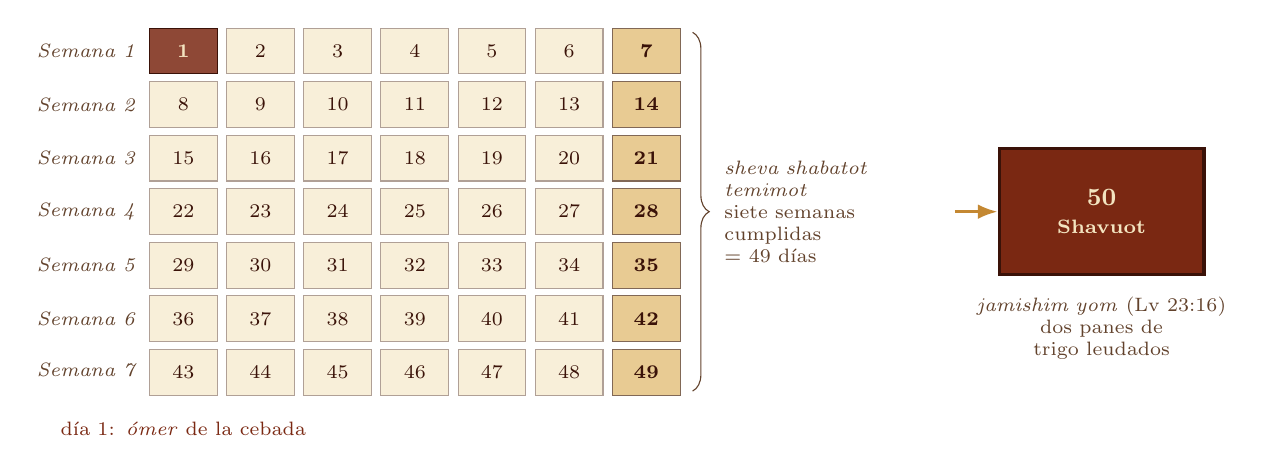
\begin{tikzpicture}[x=0.98cm,y=0.68cm]
 \foreach \w in {1,...,7}{
  \node[font=\scriptsize\itshape,text=sepia,anchor=east] at (0.5,-\w) {Semana \w};
  \foreach \d in {1,...,7}{
    \pgfmathtruncatemacro{\n}{(\w-1)*7+\d}
    \ifnum\n=1
      \node[draw=caferojizo,fill=tierraroja!85,text=papiro,minimum width=0.86cm,minimum height=0.58cm,font=\scriptsize\bfseries] at (\d,-\w) {\n};
    \else\ifnum\d=7
      \node[draw=sepia!80,fill=mostaza!55,text=caferojizo,minimum width=0.86cm,minimum height=0.58cm,font=\scriptsize\bfseries] at (\d,-\w) {\n};
    \else
      \node[draw=sepia!50,fill=papiro!60,text=caferojizo,minimum width=0.86cm,minimum height=0.58cm,font=\scriptsize] at (\d,-\w) {\n};
    \fi\fi}}
 \draw[decorate,decoration={brace,amplitude=6pt},sepia] (7.6,-0.65) -- (7.6,-7.35) node[midway,right=8pt,font=\scriptsize,text width=2.6cm,align=left]{\emph{sheva shabatot temimot}\\ siete semanas cumplidas\\ = 49 días};
 \node[draw=caferojizo,line width=1.2pt,fill=tierraroja,text=papiro,minimum width=2.6cm,minimum height=1.6cm,align=center,font=\small\bfseries] (s) at (12.9,-4) {50\\[-1pt]{\scriptsize Shavuot}};
 \draw[-{Latex[length=2.5mm]},line width=1pt,mostaza!80!tierraroja] (11.0,-4) -- (s.west);
 \node[below=4pt of s,font=\scriptsize,text width=3.2cm,align=center,text=sepia] {\emph{jamishim yom} (Lv 23:16)\\ dos panes de trigo leudados};
 \node[font=\scriptsize,text width=3.2cm,align=center,text=tierraroja] at (1,-8.05) {día 1: \emph{ómer} de la cebada};
\end{tikzpicture}}\par
\scriptsize\RaggedRight El \destacar{Jubileo} sigue el mismo esquema: ``siete semanas de años, siete veces siete años'' y el año cincuenta, santo (Lv 25:8--10). Shavuot sería un jubileo pequeño, contado en días.
\end{frame}

% ------------------------------------------------------------------
\section{Historia}

\begin{frame}{El año agrícola y sus lluvias}
\centering
\resizebox{\linewidth}{!}{%
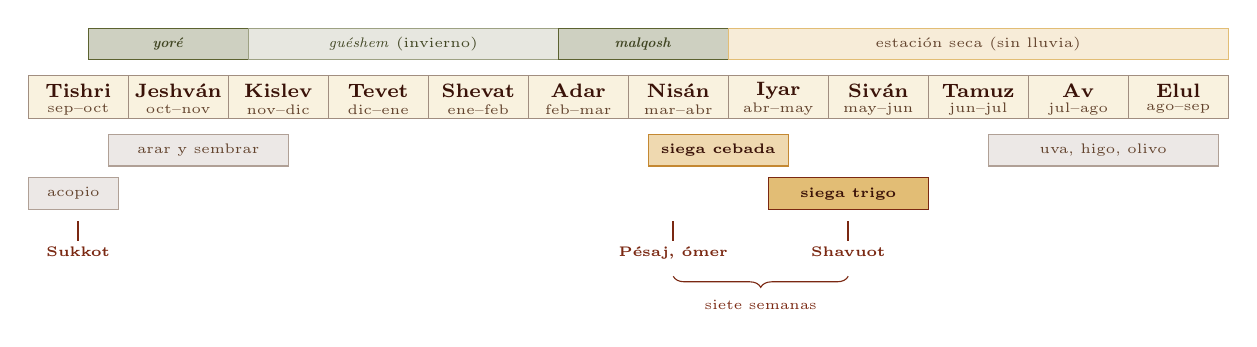
\begin{tikzpicture}[x=1.27cm,y=1cm,font=\scriptsize]
 \foreach \i/\m/\g in {0/Tishri/sep--oct,1/Jeshván/oct--nov,2/Kislev/nov--dic,3/Tevet/dic--ene,4/Shevat/ene--feb,5/Adar/feb--mar,6/Nisán/mar--abr,7/Iyar/abr--may,8/Siván/may--jun,9/Tamuz/jun--jul,10/Av/jul--ago,11/Elul/ago--sep}{
   \draw[sepia!60,fill=papiro!50] (\i,0) rectangle (\i+1,0.55);
   \node[font=\scriptsize\bfseries,text=caferojizo] at (\i+0.5,0.36) {\m};
   \node[font=\tiny,text=sepia] at (\i+0.5,0.12) {\g};}
 \fill[oliva!30,draw=oliva] (0.6,0.75) rectangle (2.2,1.15); \node[font=\tiny\bfseries,text=oliva!70!black] at (1.4,0.95) {\emph{yoré}};
 \fill[oliva!15,draw=oliva!60] (2.2,0.75) rectangle (5.3,1.15); \node[font=\tiny,text=oliva!70!black] at (3.75,0.95) {\emph{guéshem} (invierno)};
 \fill[oliva!30,draw=oliva] (5.3,0.75) rectangle (7.0,1.15); \node[font=\tiny\bfseries,text=oliva!70!black] at (6.15,0.95) {\emph{malqosh}};
 \fill[mostaza!20,draw=mostaza!70] (7.0,0.75) rectangle (12,1.15); \node[font=\tiny,text=sepia] at (9.5,0.95) {estación seca (sin lluvia)};
 \fill[sepia!12,draw=sepia!50] (0.8,-0.2) rectangle (2.6,-0.6); \node[font=\tiny,text=sepia] at (1.7,-0.4) {arar y sembrar};
 \fill[mostaza!40,draw=mostaza!80!tierraroja] (6.2,-0.2) rectangle (7.6,-0.6); \node[font=\tiny\bfseries,text=caferojizo] at (6.9,-0.4) {siega cebada};
 \fill[mostaza!70,draw=tierraroja] (7.4,-0.75) rectangle (9.0,-1.15); \node[font=\tiny\bfseries,text=caferojizo] at (8.2,-0.95) {siega trigo};
 \fill[sepia!12,draw=sepia!50] (9.6,-0.2) rectangle (11.9,-0.6); \node[font=\tiny,text=sepia] at (10.75,-0.4) {uva, higo, olivo};
 \fill[sepia!12,draw=sepia!50] (0,-0.75) rectangle (0.9,-1.15); \node[font=\tiny,text=sepia] at (0.45,-0.95) {acopio};
 \foreach \x/\t in {6.45/{Pésaj, ómer},8.2/{Shavuot},0.5/{Sukkot}}{
   \draw[tierraroja,line width=0.8pt] (\x,-1.3) -- (\x,-1.55);
   \node[below,font=\tiny\bfseries,text=tierraroja] at (\x,-1.5) {\t};}
 \draw[decorate,decoration={brace,amplitude=4pt,mirror},tierraroja] (6.45,-2.0) -- (8.2,-2.0) node[midway,below=5pt,font=\tiny,text=tierraroja]{siete semanas};
\end{tikzpicture}}\par\medskip
\begin{columns}[t,onlytextwidth]
\begin{column}{0.5\textwidth}\scriptsize\RaggedRight
La cebada madura primero; el trigo, después: ``eran tardíos'' (Éx 9:31--32). El \emph{Calendario de Gézer} (s.~\textsc{x} a.\,e.\,c.): ``mes de la siega de la cebada'', ``mes de la siega y la medida'' (Borowski, 1987).
\end{column}
\begin{column}{0.48\textwidth}\scriptsize\RaggedRight
Shavuot cae en la \destacar{estación seca}, y una lluvia en plena siega del trigo era un prodigio:``¿No es ahora la siega del trigo? Yo clamaré a \SENOR, y él dará truenos (\heb{קֹלוֹת}) y lluvias'' (1~S 12:17; cf. Pr 26:1).
\end{column}
\end{columns}
\end{frame}

\begin{frame}{Rut: la fiesta en una historia}
\begin{columns}[c,onlytextwidth]
\begin{column}{0.53\textwidth}
\centering\heb{וַתְּלַקֵּט בַּשָּׂדֶה אַחֲרֵי הַקֹּצְרִים}
\begin{cita}Fue, pues, y llegando, espigó en el campo en pos de los segadores.\fuente{(Rt 2:3a)}\end{cita}
\small\RaggedRight Rut llega ``al comienzo de la siega de la cebada'' (1:22) y espiga ``hasta que se acabó la siega de la cebada y la de trigo'' (2:23), es decir, durante \destacar{las siete semanas}.
\end{column}
\begin{column}{0.45\textwidth}\small
\begin{itemize}
\item Vive del \emph{léqet} (\heb{לָקַט}) de Lv 23:22, como \destacar{viuda pobre y extranjera}.
\item Booz da más de lo que la ley exige (2:15--16).
\item La extranjera se incorpora a Israel y llega a ser bisabuela de David (4:17).
\end{itemize}\smallskip
\precision{la lectura de Rut en Shavuot es costumbre judía posterior (\emph{Soferim} 14:3, s. \textsc{viii}); el vínculo Rut--Lv 23:22 sí es bíblico.}
\end{column}
\end{columns}
\end{frame}

\begin{frame}{Sinaí y Shavuot: lo que dice el texto}
\begin{columns}[t,onlytextwidth]
\begin{column}{0.47\textwidth}
\centering\heb{בַּחֹדֶשׁ הַשְּׁלִישִׁי}\par
\begin{cita}En el mes tercero de la salida de los hijos de Israel de la tierra de Egipto, en el mismo día llegaron al desierto de Sinaí.\fuente{(Éx 19:1)}\end{cita}
\scriptsize\RaggedRight Salida: 15 del mes primero (Nm 33:3); llegada en el mes tercero; tres días de preparación (19:10--16). La suma ronda los \destacar{cincuenta días}, aunque \destacar{el texto no fecha la Ley en Shavuot}.
\end{column}
\begin{column}{0.51\textwidth}
\begin{tcolorbox}[colback=mostaza!10,colframe=mostaza!85!tierraroja,boxrule=0.6pt,arc=2pt,left=4pt,right=4pt,top=2pt,bottom=2pt,fonttitle=\bfseries\scriptsize,coltitle=caferojizo,colbacktitle=mostaza!30,title={Precisión: ¿desde cuándo es la fiesta del Sinaí?}]
\scriptsize\RaggedRight
\textbf{Jubileos} (s.~\textsc{ii} a.\,e.\,c.): fiesta anual de renovación del pacto; Moisés sube ``en el tercer mes'' (Jub 1:1; 6:17--21).\\
\textbf{Qumrán}: renovación del pacto (1QS 1:16--2:25); reunión ``en el mes tercero'' (4Q266 11).\\
\textbf{Talmud}: ¿6 o 7 de Siván? (b. Shabbat 86b); ``el día en que fue dada la Torá'' (b. Pesajim 68b).\\[2pt]
La serie habla de ``conmemorar el día de la data de la Ley''. Esa lectura es \destacar{compatible} con Éx 19:1 y \destacar{antigua}, pero la Torá no la formula.
\end{tcolorbox}
\end{column}
\end{columns}
\end{frame}

\begin{frame}{La diáspora reunida (Hch 2:9--11)}
\begin{columns}[c,onlytextwidth]
\begin{column}{0.66\textwidth}
\resizebox{\linewidth}{!}{%
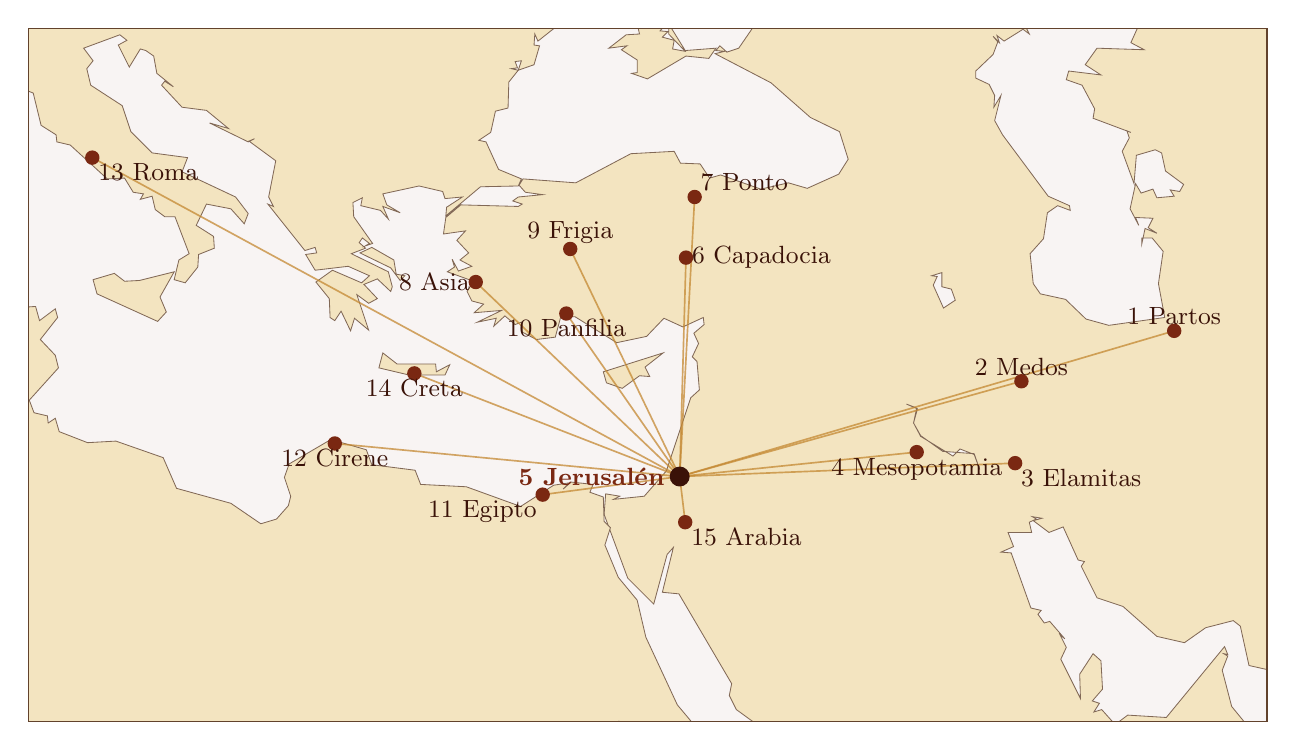
\begin{tikzpicture}[x=1cm,y=1cm,tierra/.style={fill=papiro,draw=sepia!80,line width=0.3pt},lago/.style={fill=tierraroja!5!white,draw=sepia!80,line width=0.3pt}]
\begin{scope}
\clip (0,0) rectangle (15.73,8.8);
\fill[tierraroja!5!white] (0,0) rectangle (15.73,8.8);
\fill[tierra] (16.71,0.44) -- (15.50,0.71) -- (15.39,1.21) -- (15.30,1.28) -- (14.95,1.19) -- (14.68,1.00) -- (14.33,1.08) -- (13.90,1.46) -- (13.57,1.57) -- (13.37,1.97) -- (13.41,2.03) -- (13.33,2.05) -- (13.14,2.47) -- (12.96,2.40) -- (12.76,2.55) -- (12.87,2.58) -- (12.75,2.60) -- (12.80,2.57) -- (12.71,2.53) -- (12.74,2.40) -- (12.44,2.40) -- (12.51,2.22) -- (12.35,2.15) -- (12.48,2.14) -- (12.73,1.44) -- (12.86,1.41) -- (12.82,1.36) -- (12.90,1.25) -- (12.97,1.27) -- (13.16,1.05) -- (13.10,1.10) -- (13.18,0.94) -- (13.11,0.79) -- (13.36,0.29) -- (13.35,0.60) -- (13.52,0.86) -- (13.62,0.77) -- (13.64,0.41) -- (13.51,0.26) -- (13.60,0.23) -- (13.53,0.12) -- (13.63,0.15) -- (13.80,-0.04) -- (13.96,0.08) -- (14.45,0.05) -- (15.19,0.95) -- (15.23,0.85) -- (15.18,0.86) -- (15.23,0.83) -- (15.16,0.65) -- (15.28,0.19) -- (15.46,-0.03) -- (15.97,-0.19) -- (16.22,-0.58) -- (16.32,-0.59) -- (16.17,-1.03) -- (15.90,-1.20) -- (15.80,-1.20) -- (15.65,-1.20) -- (9.99,-1.20) -- (9.74,-1.20) -- (9.57,-1.17) -- (9.48,-0.79) -- (9.55,-0.64) -- (9.32,-0.09) -- (8.99,0.15) -- (8.90,0.33) -- (8.93,0.48) -- (8.26,1.62) -- (8.05,1.64) -- (8.19,2.21) -- (8.11,2.12) -- (7.94,1.49) -- (7.61,1.82) -- (7.31,2.63) -- (7.33,2.89) -- (7.51,2.86) -- (7.43,2.82) -- (7.82,2.86) -- (8.10,3.18) -- (8.41,4.11) -- (8.52,4.21) -- (8.49,4.57) -- (8.43,4.63) -- (8.51,4.80) -- (8.45,4.93) -- (8.58,5.04) -- (8.57,5.13) -- (8.31,5.01) -- (8.07,5.12) -- (7.85,4.89) -- (7.47,4.81) -- (6.94,5.14) -- (6.76,5.14) -- (6.69,4.88) -- (6.45,4.85) -- (6.26,4.95) -- (6.26,5.07) -- (6.18,5.04) -- (6.05,5.15) -- (5.91,5.02) -- (5.94,5.12) -- (5.70,5.07) -- (6.01,5.22) -- (5.66,5.19) -- (5.78,5.30) -- (5.63,5.34) -- (5.57,5.46) -- (5.65,5.59) -- (5.32,5.71) -- (5.41,5.77) -- (5.38,5.87) -- (5.46,5.72) -- (5.63,5.78) -- (5.48,5.86) -- (5.59,5.95) -- (5.44,6.11) -- (5.55,6.23) -- (5.27,6.19) -- (5.30,6.40) -- (5.49,6.56) -- (6.22,6.54) -- (6.27,6.57) -- (6.15,6.61) -- (6.22,6.66) -- (6.53,6.69) -- (6.31,6.72) -- (6.23,6.81) -- (6.28,6.89) -- (6.95,6.84) -- (7.65,7.21) -- (8.20,7.24) -- (8.28,7.09) -- (8.53,7.08) -- (8.65,6.90) -- (8.79,6.94) -- (9.30,6.76) -- (9.65,6.84) -- (9.89,6.77) -- (10.29,6.95) -- (10.41,7.14) -- (10.30,7.49) -- (9.93,7.67) -- (9.43,8.11) -- (8.72,8.48) -- (8.84,8.51) -- (8.73,8.52) -- (8.78,8.58) -- (8.87,8.50) -- (9.02,8.55) -- (9.26,8.90) -- (9.37,8.81) -- (9.07,9.08) -- (9.37,9.06) -- (9.32,9.14) -- (9.60,9.21) -- (9.59,9.30) -- (9.03,9.24) -- (8.56,9.00) -- (8.61,9.05) -- (8.49,9.06) -- (8.19,8.83) -- (8.31,8.94) -- (8.25,9.01) -- (8.02,8.77) -- (8.12,8.76) -- (8.05,8.69) -- (8.20,8.65) -- (8.18,8.54) -- (8.34,8.51) -- (8.13,8.73) -- (8.13,8.86) -- (8.34,8.52) -- (8.73,8.55) -- (8.64,8.42) -- (8.35,8.45) -- (7.86,8.16) -- (7.66,8.23) -- (7.73,8.24) -- (7.73,8.40) -- (7.53,8.53) -- (7.60,8.58) -- (7.37,8.55) -- (7.59,8.72) -- (7.76,8.73) -- (7.73,8.86) -- (7.39,8.83) -- (7.14,8.91) -- (7.22,8.98) -- (7.05,9.03) -- (7.31,8.99) -- (7.20,9.16) -- (7.14,9.04) -- (7.02,9.05) -- (7.07,9.14) -- (7.02,9.05) -- (6.80,9.02) -- (6.71,8.83) -- (6.60,8.95) -- (6.71,8.83) -- (6.47,8.64) -- (6.43,8.73) -- (6.42,8.59) -- (6.49,8.58) -- (6.42,8.34) -- (6.22,8.27) -- (6.26,8.39) -- (6.18,8.38) -- (6.21,8.30) -- (6.13,8.29) -- (6.22,8.27) -- (6.10,8.12) -- (6.09,7.79) -- (5.93,7.75) -- (5.87,7.48) -- (5.72,7.38) -- (5.81,7.36) -- (5.97,7.01) -- (6.26,6.89) -- (6.22,6.80) -- (5.74,6.79) -- (5.30,6.42) -- (5.31,6.53) -- (5.51,6.66) -- (5.29,6.64) -- (5.26,6.73) -- (4.96,6.80) -- (4.50,6.70) -- (4.55,6.56) -- (4.72,6.46) -- (4.50,6.54) -- (4.57,6.38) -- (4.47,6.49) -- (4.22,6.55) -- (4.24,6.65) -- (4.12,6.59) -- (4.13,6.41) -- (4.37,6.07) -- (4.28,6.04) -- (4.33,6.07) -- (4.24,6.14) -- (4.20,6.08) -- (4.28,6.01) -- (4.10,5.94) -- (4.57,5.71) -- (4.62,5.52) -- (4.60,5.46) -- (4.43,5.62) -- (4.26,5.55) -- (4.43,5.37) -- (4.32,5.31) -- (4.17,5.42) -- (4.32,4.97) -- (4.14,5.12) -- (4.09,4.96) -- (3.97,5.21) -- (3.89,5.09) -- (3.83,5.13) -- (3.82,5.37) -- (3.65,5.58) -- (3.86,5.73) -- (4.23,5.57) -- (4.33,5.66) -- (4.06,5.78) -- (3.64,5.73) -- (3.52,5.93) -- (3.66,5.95) -- (3.64,6.02) -- (3.51,5.98) -- (3.04,6.57) -- (3.11,6.54) -- (3.05,6.66) -- (3.14,7.12) -- (2.80,7.37) -- (2.87,7.40) -- (2.79,7.36) -- (2.30,7.60) -- (2.54,7.53) -- (2.26,7.76) -- (1.95,7.80) -- (1.69,8.08) -- (1.73,8.13) -- (1.84,8.06) -- (1.63,8.23) -- (1.59,8.45) -- (1.49,8.52) -- (1.42,8.54) -- (1.28,8.31) -- (1.14,8.59) -- (1.25,8.65) -- (1.16,8.72) -- (0.70,8.55) -- (0.82,8.39) -- (0.74,8.29) -- (0.79,8.08) -- (1.19,7.82) -- (1.30,7.49) -- (1.57,7.22) -- (2.02,7.16) -- (1.95,6.98) -- (2.63,6.66) -- (2.79,6.45) -- (2.74,6.32) -- (2.57,6.51) -- (2.26,6.57) -- (2.13,6.30) -- (2.35,6.16) -- (2.36,6.01) -- (2.16,5.93) -- (2.15,5.77) -- (1.99,5.57) -- (1.85,5.61) -- (1.91,5.86) -- (2.04,5.94) -- (1.86,6.41) -- (1.73,6.41) -- (1.61,6.50) -- (1.57,6.67) -- (1.42,6.63) -- (1.46,6.70) -- (1.33,6.72) -- (1.22,6.90) -- (1.00,6.89) -- (0.53,7.32) -- (0.36,7.36) -- (0.35,7.45) -- (0.16,7.57) -- (0.06,7.98) -- (-0.41,8.17) -- (-0.63,7.96) -- (-0.92,7.88) -- (-0.98,7.67) -- (-0.98,7.64) -- (-0.98,10.00) -- (16.71,10.00) -- (16.71,0.44) -- cycle;
\fill[tierra] (7.30,2.85) -- (7.31,2.54) -- (7.39,2.46) -- (7.32,2.24) -- (7.49,1.83) -- (7.73,1.54) -- (7.84,1.07) -- (8.24,0.21) -- (8.45,-0.04) -- (8.35,-0.03) -- (8.41,-0.42) -- (8.81,-0.77) -- (8.84,-1.04) -- (8.95,-1.17) -- (8.88,-1.11) -- (8.91,-1.20) -- (-0.98,-1.20) -- (-0.98,5.15) -- (-0.98,5.21) -- (-0.98,5.15) -- (-0.86,5.23) -- (-0.69,5.14) -- (-0.08,5.34) -- (-0.06,5.26) -- (0.09,5.27) -- (0.14,5.09) -- (0.34,5.24) -- (0.37,5.13) -- (0.15,4.85) -- (0.34,4.65) -- (0.38,4.49) -- (0.01,4.08) -- (0.07,3.92) -- (0.24,3.88) -- (0.25,3.79) -- (0.34,3.85) -- (0.39,3.68) -- (0.75,3.54) -- (1.11,3.56) -- (1.71,3.35) -- (1.88,2.96) -- (2.57,2.77) -- (2.95,2.51) -- (3.15,2.57) -- (3.30,2.74) -- (3.33,2.86) -- (3.25,3.10) -- (3.31,3.27) -- (3.84,3.58) -- (4.29,3.45) -- (4.36,3.26) -- (4.91,3.19) -- (4.98,3.01) -- (5.56,2.98) -- (6.25,2.73) -- (6.67,3.00) -- (6.87,3.03) -- (6.79,2.95) -- (6.89,3.04) -- (7.17,3.01) -- (7.13,2.91) -- (7.30,2.85) -- cycle;
\fill[tierra] (1.64,5.08) -- (0.87,5.43) -- (0.82,5.61) -- (1.09,5.69) -- (1.22,5.59) -- (1.41,5.60) -- (1.85,5.71) -- (1.67,5.39) -- (1.75,5.20) -- (1.64,5.08) -- cycle;
\fill[tierra] (-0.51,6.00) -- (-0.47,6.33) -- (-0.60,6.78) -- (-0.47,6.73) -- (-0.25,6.90) -- (-0.16,6.86) -- (-0.06,6.61) -- (-0.12,6.50) -- (-0.12,6.12) -- (-0.16,6.04) -- (-0.32,6.11) -- (-0.37,5.95) -- (-0.51,6.00) -- cycle;
\fill[tierra] (7.54,4.23) -- (7.34,4.30) -- (7.30,4.44) -- (8.06,4.68) -- (7.83,4.50) -- (7.89,4.38) -- (7.76,4.39) -- (7.54,4.23) -- cycle;
\fill[tierra] (-0.33,6.99) -- (-0.44,7.10) -- (-0.39,7.16) -- (-0.46,7.16) -- (-0.41,7.22) -- (-0.48,7.35) -- (-0.23,7.47) -- (-0.19,7.61) -- (-0.15,7.25) -- (-0.26,6.95) -- (-0.33,6.99) -- cycle;
\fill[tierra] (4.83,4.40) -- (4.45,4.49) -- (4.50,4.68) -- (4.68,4.54) -- (5.17,4.54) -- (5.18,4.44) -- (5.35,4.53) -- (5.29,4.40) -- (4.83,4.40) -- cycle;
\fill[tierra] (4.72,5.60) -- (4.60,5.76) -- (4.21,5.95) -- (4.36,6.02) -- (4.64,5.86) -- (4.67,5.68) -- (4.78,5.66) -- (4.72,5.60) -- cycle;
\fill[lago] (12.89,6.13) -- (12.94,6.46) -- (13.07,6.55) -- (13.23,6.49) -- (13.22,6.55) -- (12.95,6.67) -- (12.37,7.45) -- (12.27,7.63) -- (12.35,7.95) -- (12.26,7.80) -- (12.27,7.95) -- (12.20,8.09) -- (12.03,8.17) -- (12.03,8.26) -- (12.25,8.47) -- (12.31,8.63) -- (12.25,8.70) -- (12.33,8.62) -- (12.30,8.71) -- (12.39,8.64) -- (12.63,8.79) -- (12.71,8.73) -- (12.66,8.83) -- (12.88,8.90) -- (12.88,9.03) -- (13.04,9.01) -- (13.50,9.25) -- (13.83,9.12) -- (13.91,9.20) -- (14.11,9.16) -- (14.14,8.93) -- (14.00,8.62) -- (14.17,8.53) -- (13.57,8.55) -- (13.42,8.34) -- (13.62,8.21) -- (13.21,8.26) -- (13.18,8.15) -- (13.38,8.08) -- (13.54,7.78) -- (13.52,7.66) -- (14.00,7.48) -- (13.95,7.50) -- (13.98,7.41) -- (13.89,7.24) -- (14.04,6.83) -- (14.07,7.19) -- (14.31,7.26) -- (14.39,7.22) -- (14.44,6.99) -- (14.67,6.82) -- (14.62,6.73) -- (14.50,6.75) -- (14.55,6.67) -- (14.33,6.65) -- (14.28,6.76) -- (14.13,6.71) -- (14.06,6.83) -- (13.99,6.51) -- (14.10,6.30) -- (14.06,6.40) -- (14.28,6.39) -- (14.22,6.27) -- (14.33,6.20) -- (14.18,6.26) -- (14.14,6.07) -- (14.14,6.14) -- (14.27,6.14) -- (14.41,5.97) -- (14.35,5.56) -- (14.43,5.13) -- (13.72,5.03) -- (13.43,5.11) -- (13.17,5.36) -- (12.85,5.43) -- (12.76,5.56) -- (12.72,5.94) -- (12.89,6.13) -- cycle;
\fill[lago] (16.71,8.29) -- (16.71,8.26) -- (16.71,8.04) -- (16.70,8.13) -- (16.62,8.01) -- (16.71,7.85) -- (16.30,7.76) -- (16.32,7.86) -- (15.98,7.98) -- (16.05,7.87) -- (15.87,7.85) -- (15.79,8.34) -- (15.95,8.73) -- (16.18,8.82) -- (16.15,8.70) -- (16.22,8.73) -- (16.20,8.92) -- (16.30,8.94) -- (16.35,8.84) -- (16.42,8.91) -- (16.31,9.01) -- (16.49,9.09) -- (16.58,9.03) -- (16.54,9.12) -- (16.67,9.11) -- (16.65,9.03) -- (16.71,8.99) -- (16.71,9.15) -- (16.71,9.10) -- (16.71,8.86) -- (16.68,8.84) -- (16.71,8.76) -- (16.69,8.66) -- (16.71,8.71) -- (16.71,8.46) -- (16.71,8.42) -- (16.71,8.29) -- cycle;
\fill[lago] (7.16,10.00) -- (7.43,10.00) -- (7.61,10.00) -- (7.90,9.97) -- (8.11,9.80) -- (8.28,9.85) -- (8.21,9.64) -- (8.29,9.37) -- (7.88,9.36) -- (7.93,9.32) -- (7.77,9.14) -- (7.42,9.06) -- (7.72,9.14) -- (7.84,9.42) -- (8.19,9.42) -- (8.24,9.70) -- (8.21,9.78) -- (7.66,10.00) -- (7.53,9.99) -- (7.16,10.00) -- cycle;
\fill[lago] (11.60,5.70) -- (11.60,5.52) -- (11.72,5.49) -- (11.77,5.35) -- (11.62,5.25) -- (11.49,5.54) -- (11.54,5.65) -- (11.47,5.66) -- (11.60,5.70) -- cycle;
\fill[lago] (7.50,-0.01) -- (7.55,-0.19) -- (7.49,-0.35) -- (7.56,-0.44) -- (7.45,-0.38) -- (7.32,-0.59) -- (7.22,-0.53) -- (6.89,-1.00) -- (7.15,-0.61) -- (7.10,-0.54) -- (7.39,-0.49) -- (7.51,-0.28) -- (7.49,-0.19) -- (7.41,-0.20) -- (7.48,-0.18) -- (7.50,-0.01) -- cycle;
\fill[lago] (11.06,10.00) -- (11.15,10.00) -- (10.97,9.90) -- (11.07,9.87) -- (10.86,9.71) -- (10.84,9.48) -- (10.81,9.54) -- (10.54,9.41) -- (10.61,9.57) -- (10.55,9.60) -- (10.74,9.55) -- (10.73,9.66) -- (10.84,9.73) -- (10.79,9.82) -- (10.93,9.78) -- (10.96,9.91) -- (11.11,9.99) -- (11.14,10.00) -- (11.04,10.00) -- (11.00,10.00) -- (11.06,10.00) -- cycle;
\fill[lago] (11.33,9.81) -- (11.28,9.84) -- (11.45,10.00) -- (11.61,10.00) -- (11.33,9.81) -- cycle;
\fill[lago] (11.15,4.03) -- (11.29,3.97) -- (11.24,3.79) -- (11.33,3.63) -- (11.61,3.43) -- (12.01,3.40) -- (12.08,3.20) -- (12.01,3.39) -- (11.83,3.46) -- (11.74,3.37) -- (11.33,3.62) -- (11.24,3.79) -- (11.28,3.98) -- (11.15,4.03) -- cycle;
\end{scope}
\draw[sepia,line width=0.6pt] (0,0) rectangle (15.73,8.8);
\coordinate (J) at (8.27,3.11);
\foreach \p in {(14.55,4.96),(12.61,4.32),(12.53,3.28),(11.28,3.42),(8.35,5.89),(8.46,6.66),(5.68,5.58),(6.88,6.00),(6.83,5.18),(6.53,2.88),(3.89,3.53),(0.81,7.16),(4.90,4.42),(8.34,2.53)}
  \draw[mostaza!80!tierraroja,line width=0.6pt,opacity=0.75] (J) -- \p;
\foreach \p/\n/\pos in {(14.55,4.96)/{1 Partos}/above,(12.61,4.32)/{2 Medos}/above,(12.53,3.28)/{3 Elamitas}/below right,(11.28,3.42)/{4 Mesopotamia}/below,(8.35,5.89)/{6 Capadocia}/right,(8.46,6.66)/{7 Ponto}/above right,(5.68,5.58)/{8 Asia}/left,(6.88,6.00)/{9 Frigia}/above,(6.83,5.18)/{10 Panfilia}/below,(6.53,2.88)/{11 Egipto}/below left,(3.89,3.53)/{12 Cirene}/below,(0.81,7.16)/{13 Roma}/below right,(4.90,4.42)/{14 Creta}/below,(8.34,2.53)/{15 Arabia}/below right}{
  \fill[tierraroja] \p circle (2.6pt);
  \node[\pos,font=\small,text=caferojizo,inner sep=2pt] at \p {\n};}
\fill[caferojizo] (J) circle (3.6pt); \node[left=2pt,font=\small\bfseries,text=tierraroja] at (J) {5 Jerusalén};
\end{tikzpicture}}\par
{\fontsize{4.5}{5.5}\selectfont\color{sepia}\textit{Nota.} Elaboración propia; costas simplificadas (GSHHS) y ubicaciones aproximadas por coordenadas reales.\par}
\end{column}
\begin{column}{0.32\textwidth}\scriptsize\RaggedRight
``Partos, medos, elamitas\ldots{} cretenses y árabes, les oímos hablar en nuestras lenguas las maravillas de Dios'' (Hch 2:9--11).\par\medskip
La lista va de oriente (los deportados de Asiria y Babilonia, 2~R 17:6) a occidente (Roma). Unos la leen sobre Gn 10 (Scott, 1994); otros, como inventario de la diáspora (Fitzmyer, 1998).
\end{column}
\end{columns}
\end{frame}

\begin{frame}{Shavuot en la historia y peregrinación}
\centering
\resizebox{\linewidth}{!}{%
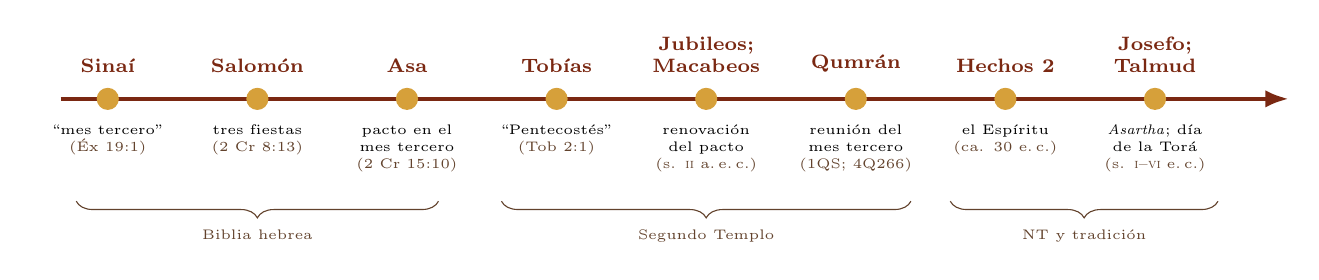
\begin{tikzpicture}[font=\scriptsize]
 \draw[line width=1.6pt,tierraroja,-{Latex[length=3mm]}] (0,0) -- (15.6,0);
 \foreach \x/\a/\b/\c in {0.6/{Sinaí}/{``mes tercero''}/{Éx 19:1},2.5/{Salomón}/{tres fiestas}/{2 Cr 8:13},4.4/{Asa}/{pacto en el mes tercero}/{2 Cr 15:10},6.3/{Tobías}/{``Pentecostés''}/{Tob 2:1},8.2/{Jubileos; Macabeos}/{renovación del pacto}/{s. \textsc{ii} a.\,e.\,c.},10.1/{Qumrán}/{reunión del mes tercero}/{1QS; 4Q266},12.0/{Hechos 2}/{el Espíritu}/{ca. 30 e.\,c.},13.9/{Josefo; Talmud}/{\emph{Asartha}; día de la Torá}/{s. \textsc{i}--\textsc{vi} e.\,c.}}{
   \fill[mostaza] (\x,0) circle (4pt);
   \node[above=6pt,font=\scriptsize\bfseries,text=tierraroja,text width=1.8cm,align=center] at (\x,0) {\a};
   \node[below=6pt,text width=1.8cm,align=center,font=\tiny] at (\x,0) {\b\\ \textcolor{sepia}{(\c)}};}
 \draw[decorate,decoration={brace,amplitude=6pt,mirror},sepia] (0.2,-1.3) -- (4.8,-1.3) node[midway,below=7pt,font=\tiny,text=sepia] {Biblia hebrea};
 \draw[decorate,decoration={brace,amplitude=6pt,mirror},sepia] (5.6,-1.3) -- (10.8,-1.3) node[midway,below=7pt,font=\tiny,text=sepia] {Segundo Templo};
 \draw[decorate,decoration={brace,amplitude=6pt,mirror},sepia] (11.3,-1.3) -- (14.7,-1.3) node[midway,below=7pt,font=\tiny,text=sepia] {NT y tradición};
\end{tikzpicture}}\par\medskip
\scriptsize\RaggedRight\begin{itemize}
\item Asa reúne a Judá ``en el mes tercero'': pacto, alegría y ``juramento'' (\heb{הַשְּׁבוּעָה}, 2~Cr 15:10--15) \precision{inferencia (Weinfeld, 1978): no nombra la fiesta}.
\item Tobías: ``la fiesta de Pentecostés, que es la santa fiesta de las siete semanas'' (Tob 2:1); 2 Mac 12:31--32 \precision{deuterocanónicos}.
\item Josefo: ``el día que los hebreos llaman \emph{Asartha}, que significa Pentecostés'' (\emph{Ant.} 3.252); multitudes en Jerusalén en el 4 a.\,e.\,c. (\emph{Guerra} 2.42--44).
\end{itemize}
\end{frame}

% ------------------------------------------------------------------
\section{Filología}

\begin{frame}{Semanas, siete y juramento}
\begin{columns}[t,onlytextwidth]
\begin{column}{0.55\textwidth}
\scriptsize\renewcommand{\arraystretch}{1.12}
\begin{tabular}{@{}L{2.2cm}L{4.4cm}@{}}
\toprule
\textbf{Palabra} & \textbf{Sentido} \\ \midrule
\heb{שֶׁבַע} \emph{sheva} & ``siete''; \heb{שְׁבִיעִי} ``séptimo'' \\
\heb{שָׁבוּעַ} \emph{shavúa} & ``semana'', unidad de siete (Dn 9:24--27) \\
\heb{חַג שָׁבֻעוֹת} & ``fiesta de las semanas''; \emph{jag}: peregrinación \\
\heb{שְׁבוּעָה} \emph{shevuá} & ``juramento''; ``semanas'' y ``juramentos'' se escriben igual: \heb{שבעות} \\
\heb{שַׁבָּתוֹת} \emph{shabatot} & en Lv 23:15 las semanas se llaman ``sábados'' \\
\bottomrule
\end{tabular}
\end{column}
\begin{column}{0.43\textwidth}\small\RaggedRight
El juego ``semanas / juramentos'' es \destacar{homilético} y del judaísmo posterior; la vocalización distingue ambas palabras.\par\medskip
Jeremías une las dos lluvias y las semanas: el \SENOR{} ``da lluvia temprana y tardía en su tiempo, y nos guarda los tiempos establecidos de la siega'' (Jer 5:24): \heb{שְׁבֻעֹת חֻקּוֹת קָצִיר}, ``las semanas fijadas de la siega''.
\end{column}
\end{columns}
\end{frame}

\begin{frame}{Contar, cumplir, primicias}
\scriptsize\renewcommand{\arraystretch}{1.15}
\begin{tabular}{@{}L{2.9cm}L{1.1cm}L{7.8cm}@{}}
\toprule
\textbf{Término} & \textbf{Raíz} & \textbf{Sentido y usos} \\ \midrule
\heb{וּסְפַרְתֶּם} \emph{usfartem} & \heb{ספר} & ``y contaréis''; la raíz de \emph{séfer} (libro). Abre también la cuenta del Jubileo (Lv 25:8) \\
\heb{תְּמִימֹת} \emph{temimot} & \heb{תמם} & ``cumplidas, completas'': el adjetivo de la víctima ``sin defecto'' (Lv 23:12, 18) \\
\heb{חֲמִשִּׁים יוֹם} \emph{jamishim yom} & \heb{חמשׁ} & ``cincuenta días''; LXX \grc{πεντήκοντα ἡμέρας} \\
\heb{מִנְחָה חֲדָשָׁה} & \heb{חדשׁ} & ``ofrenda nueva'': el adjetivo de ``pacto nuevo'' (Jer 31:31) y ``corazón nuevo'' (Ez 36:26) \\
\heb{קָצִיר} \emph{qatsir} & \heb{קצר} & ``siega'' del grano; distinta de \heb{אָסִיף} (\emph{asif}), la cosecha de otoño \\
\heb{בִּכּוּרִים} \emph{bikurim} & \heb{בכר} & ``primicias''; raíz de \emph{bejor}, primogénito \\
\heb{חִטִּים} \emph{jitim} & \heb{חטה} & ``trigo'' (Éx 34:22), frente a \heb{שְׂעֹרִים}, ``cebada'' (Rt 1:22) \\
\grc{ἀπαρχή} \emph{aparchē} & --- & ``primicia'': Cristo (1 Co 15:20); ``primicias del Espíritu'' (Ro 8:23) \\
\bottomrule
\end{tabular}
\end{frame}

\begin{frame}{Leudado, mecido y no quemado}
\begin{columns}[t,onlytextwidth]
\begin{column}{0.52\textwidth}
\begin{cita}Ninguna ofrenda que ofreciereis a \SENOR{} será con levadura\ldots{} Como ofrenda de primicias las ofreceréis a \SENOR; mas no subirán sobre el altar en olor grato.\fuente{(Lv 2:11--12)}\end{cita}
\scriptsize\RaggedRight La misma ley que prohíbe la levadura en el altar \destacar{prevé la excepción} de las primicias, con una condición: no se queman. Los panes se mecen y quedan para el sacerdote (Lv 23:20).
\end{column}
\begin{column}{0.46\textwidth}\small
\begin{itemize}
\item \heb{חָמֵץ} \emph{jamets}: lo leudado; \heb{שְׂאֹר} \emph{se'or}: la masa madre.
\item \heb{תְּנוּפָה} \emph{tenufá}: ofrenda mecida o elevada (Milgrom, 1991): \emph{ómer}, panes y corderos.
\item \heb{סֹלֶת} \emph{sólet}: flor de harina; dos décimas de efa.
\end{itemize}
\precision{Lv 2:4--5 aplica la norma a las tortas; la norma general es Lv 2:11 y la excepción, 2:12.}
\end{column}
\end{columns}
\end{frame}

\begin{frame}{El lenguaje del Sinaí}
\fotolado{panel_exodo20.jpg}{Elaboración propia: Éx 20:18 en texto hebreo consonántico (BHS).}
\begin{columns}[c,onlytextwidth]
\begin{column}{0.57\textwidth}
\begin{cita}Todo el pueblo observaba el estruendo y los relámpagos, y el sonido de la bocina, y el monte que humeaba\ldots\fuente{(Éx 20:18)}\end{cita}
\scriptsize\RaggedRight
El hebreo dice ``veían las \destacar{voces}'' (\heb{רֹאִים אֶת־הַקּוֹלֹת}); \emph{qolot} son truenos y voces (19:16). Las \emph{lapidim} (\heb{לַפִּידִם}) son ``antorchas'' (RVR: ``relámpagos''), como la ``antorcha de fuego'' de Gn 15:17. El \emph{esh} (\heb{אֵשׁ}): ``descendido sobre él en fuego'' (19:18).\par\smallskip
\textbf{Filón}: la voz del Sinaí, fuego hecho lenguaje: \grc{τῆς φλογὸς εἰς διάλεκτον ἀρθρουμένης} (\emph{De Decalogo} 33, 46).
\end{column}
\begin{column}{0.41\textwidth}\end{column}
\end{columns}
\end{frame}

\begin{frame}{El lenguaje de Hechos 2}
\fotolado{panel_hechos2.jpg}{Elaboración propia: Hch 2:1 en escritura uncial (texto NA28).}
\begin{columns}[c,onlytextwidth]
\begin{column}{0.57\textwidth}
\begin{cita}Cuando llegó el día de Pentecostés, estaban todos unánimes juntos. Y de repente vino del cielo un estruendo como de un viento recio\ldots{} y se les aparecieron lenguas repartidas, como de fuego\ldots\fuente{(Hch 2:1--3)}\end{cita}
\scriptsize\RaggedRight
\grc{ἐν τῷ συμπληροῦσθαι}: ``al \destacar{cumplirse}'' el plazo de la cuenta (cf. Lc 9:51).
\grc{ἦχος}: ``estruendo''; \grc{πνοὴ βιαία}: ``soplo violento'' (\emph{pnoē}, familia de \grc{πνεῦμα}).
\grc{γλῶσσαι ὡσεὶ πυρός}: ``lenguas \destacar{como} de fuego''.
\grc{φωνή} (v. 6): ``voz'', el griego de \emph{qol}.
\end{column}
\begin{column}{0.41\textwidth}\end{column}
\end{columns}
\end{frame}

\begin{frame}{De \emph{shavuot} a Pentecostés}
\centering
\resizebox{\linewidth}{!}{%
\begin{tikzpicture}[font=\small,node distance=0.55cm,
  bx/.style={draw=tierraroja,line width=0.8pt,fill=papiro,rounded corners=3pt,text width=3.0cm,align=center,inner sep=5pt,minimum height=2.5cm}]
 \node[bx] (h) {\textbf{Hebreo}\\ \heb{חַג שָׁבֻעוֹת}\\ \emph{jag shavuot}\\ {\footnotesize ``fiesta de las semanas''}\\ {\scriptsize\color{sepia}Éx 34:22; Dt 16:10}};
 \node[bx,right=of h] (l) {\textbf{LXX Pentateuco}\\ \grc{ἑορτὴ ἑβδομάδων}\\ {\footnotesize ``fiesta de semanas''}\\ {\scriptsize\color{sepia}Éx 34:22; Dt 16:10}};
 \node[bx,right=of l] (g) {\textbf{Griego judío}\\ \grc{πεντηκοστή}\\ {\footnotesize ``el quincuagésimo [día]''}\\ {\scriptsize\color{sepia}Tob 2:1; 2 Mac 12:32; Josefo}};
 \node[bx,right=of g,draw=mostaza,line width=1.4pt,fill=tierraroja,text=papiro] (n) {\textbf{NT}\\ \grc{ἡ ἡμέρα τῆς πεντηκοστῆς}\\ {\footnotesize ``el día de Pentecostés''}\\ {\scriptsize Hch 2:1; 20:16; 1 Co 16:8}};
 \draw[-{Latex[length=3mm]},mostaza!80!tierraroja,line width=1.3pt] (h)--(l);
 \draw[-{Latex[length=3mm]},mostaza!80!tierraroja,line width=1.3pt] (l)--(g);
 \draw[-{Latex[length=3mm]},mostaza!80!tierraroja,line width=1.3pt] (g)--(n);
\end{tikzpicture}}\par\bigskip
\small\RaggedRight El nombre pasa de la \destacar{unidad que se cuenta} (semanas) al \destacar{día al que se llega} (cincuenta). Latín \emph{Pentecoste} $\rightarrow$ español \emph{Pentecostés}. En arameo \emph{Asartha}, en la Misná \heb{עֲצֶרֶת} (\emph{atséret}), ``asamblea de clausura'' (Josefo, \emph{Ant.} 3.252).
\end{frame}

\begin{frame}{Joel 2:23: lluvia y maestro}
\fotolado{panel_joel2.jpg}{Elaboración propia: Jl 2:23b en texto hebreo consonántico (BHS).}
\begin{columns}[c,onlytextwidth]
\begin{column}{0.57\textwidth}
\begin{cita}Vosotros también, hijos de Sion, alegraos y gozaos en \SENOR{} vuestro Dios; porque os ha dado la primera lluvia a su tiempo, y hará descender sobre vosotros lluvia temprana y tardía como al principio.\fuente{(Jl 2:23, RVR1960)}\end{cita}
\scriptsize\RaggedRight
La lluvia \destacar{temprana} de otoño es \emph{yoré} o \emph{moré} (\heb{יוֹרֶה}, \heb{מוֹרֶה}; Dt 11:14); la \destacar{tardía} de primavera, \emph{malqosh} (\heb{מַלְקוֹשׁ}). \emph{Barishón} (\heb{בָּרִאשׁוֹן}) es ``en el primero'', ``como antes'' (LXX \grc{καθὼς ἔμπροσθεν}).
\end{column}
\begin{column}{0.41\textwidth}\end{column}
\end{columns}
\end{frame}

\begin{frame}{\emph{Moré litsdaká}: ¿lluvia o maestro?}
\begin{columns}[t,onlytextwidth]
\begin{column}{0.49\textwidth}
\begin{tcolorbox}[colback=oliva!8,colframe=oliva,boxrule=0.8pt,arc=2pt,left=4pt,right=4pt,fonttitle=\bfseries\small,coltitle=papiro,colbacktitle=oliva,title={(1) Lluvia}]
\scriptsize\RaggedRight Contexto agrícola (vv. 19--26); la segunda mitad del versículo usa \emph{moré} como lluvia; \emph{litsdaká} = ``en justa medida''. RVR1960 ``a su tiempo''; RV 1909 ``\destacar{arregladamente}''.
\end{tcolorbox}
\end{column}
\begin{column}{0.49\textwidth}
\begin{tcolorbox}[colback=tierraroja!6,colframe=tierraroja,boxrule=0.8pt,arc=2pt,left=4pt,right=4pt,fonttitle=\bfseries\small,coltitle=papiro,colbacktitle=tierraroja,title={(2) Maestro}]
\scriptsize\RaggedRight \emph{Hamoré} con artículo + ``para justicia'' suena a título. Vulgata \emph{doctorem iustitiae}; Ahlström (1971). Qumrán: \heb{מוֹרֵה צֶדֶק}, ``Maestro de Justicia'' (CD 1:11).
\end{tcolorbox}
\end{column}
\end{columns}\medskip
\small\RaggedRight La raíz \heb{ירה} significa ``lanzar'' (agua, flechas) y ``enseñar'' (de ahí \emph{torá}). Oseas juega con el mismo doble sentido: ``hasta que venga y os enseñe justicia'' (\heb{וְיֹרֶה צֶדֶק}, Os 10:12). La enseñanza cae como lluvia (Dt 32:2). Wolff (1977) y Crenshaw (1995) discuten ambas lecturas.
\par\smallskip\precision{Strong H4175 (\emph{moré}) cubre ``lluvia temprana'' y ``maestro''; H6666 (\emph{tsedaqá}) es ``justicia'': ``a su tiempo'' es interpretación de la RVR1960.}
\end{frame}

% ------------------------------------------------------------------
\section{Texto}

\begin{frame}{El cómputo de Lv 23:15--16}
\scriptsize\renewcommand{\arraystretch}{1.18}
\begin{tabular}{@{}L{2.3cm}L{3.5cm}L{2.3cm}L{3.4cm}@{}}
\toprule
\textbf{Lectura} & \textbf{``Sábado'' en Lv 23:11, 15} & \textbf{Shavuot cae} & \textbf{Testigos} \\ \midrule
Farisea y rabínica & primer día de Matsot (15 Nisán); \emph{shabatot} = semanas & 6 de Siván, cualquier día & LXX Lv 23:11 \grc{τῇ ἐπαύριον τῆς πρώτης}; Josefo, \emph{Ant.} 3.250; Filón \\
Saducea y caraíta & sábado semanal dentro de Matsot & siempre domingo & boetusianos (b. Menajot 65a--66a); caraítas; samaritanos \\
Jubileos y Qumrán & sábado tras la semana de Matsot (año de 364 días) & domingo 15 del mes tercero & Jub 15:1; 11QT 18--19; VanderKam (1998) \\
\bottomrule
\end{tabular}\par\medskip
\small\RaggedRight ``Siete \emph{shabatot} cumplidas'' se entiende mejor con semanas de sábado a sábado; la LXX fijó la lectura farisea. Deuteronomio cuenta desde el campo (Dt 16:9); la glosa judía: desde el 2.º día de Pésaj, con Jos 5:11 (``al otro día de la pascua'', \heb{מִמָּחֳרַת הַפֶּסַח}, comieron del fruto de la tierra).\par\smallskip
\precision{contando desde el sábado semanal, Pentecostés cae siempre en domingo. Ver estudio 3.}
\end{frame}

\begin{frame}{Precisión textual}
\begin{columns}[t,onlytextwidth]
\begin{column}{0.53\textwidth}
\scriptsize\renewcommand{\arraystretch}{1.12}
\begin{tabular}{@{}L{1.3cm}L{4.9cm}@{}}
\toprule
\textbf{Testigo} & \textbf{Jl 2:23a} \\ \midrule
TM & \heb{כִּי־נָתַן לָכֶם אֶת־הַמּוֹרֶה לִצְדָקָה} \\
LXX & \grc{ἔδωκεν ὑμῖν τὰ βρώματα εἰς δικαιοσύνην}, ``los alimentos'' \\
Vulgata & \emph{dedit vobis doctorem iustitiae} \\
RV 1909 & ``la primera lluvia arregladamente'' \\
RVR1960 & ``la primera lluvia a su tiempo'' \\
\bottomrule
\end{tabular}
\end{column}
\begin{column}{0.45\textwidth}\scriptsize\RaggedRight
\textbf{Hch 2:17}: TM \heb{אַחֲרֵי־כֵן} y LXX \grc{μετὰ ταῦτα} (``después de esto''); NA28 \grc{ἐν ταῖς ἐσχάταις ἡμέραις} (``en los postreros días''); el Códice Vaticano (B) lee \grc{μετὰ ταῦτα}. Pedro añade ``y profetizarán'' (2:18).\par\smallskip
\textbf{Hch 2:1}: NA28 ``el día''; Vulgata \emph{dies}, de donde la RV 1909: ``como se cumplieron \destacar{los días} de Pentecostés''.\par\smallskip
\textbf{Joel}: 2:28--32 = 3:1--5 en hebreo.
\end{column}
\end{columns}
\end{frame}

% ------------------------------------------------------------------
\section{Literatura}

\begin{frame}{Estructura de Lv 23:15--22}
\centering
\resizebox{\linewidth}{!}{%
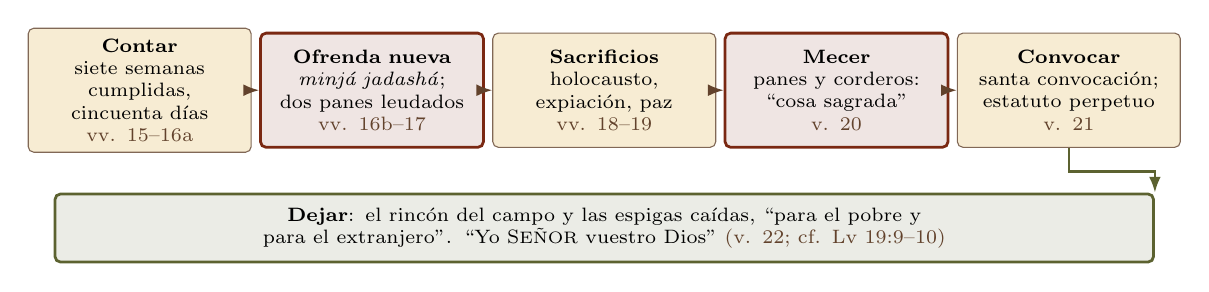
\begin{tikzpicture}[font=\scriptsize,
  bl/.style={draw=sepia!80,fill=papiro!70,rounded corners=2pt,text width=2.55cm,align=center,inner sep=4pt,minimum height=1.45cm},
  bc/.style={draw=tierraroja,line width=1pt,fill=tierraroja!12,rounded corners=2pt,text width=2.55cm,align=center,inner sep=4pt,minimum height=1.45cm}]
 \node[bl] (a) at (0,0) {\textbf{Contar}\\ siete semanas cumplidas, cincuenta días\\ {\color{sepia}vv. 15--16a}};
 \node[bc] (b) at (2.95,0) {\textbf{Ofrenda nueva}\\ \emph{minjá jadashá}; dos panes leudados\\ {\color{sepia}vv. 16b--17}};
 \node[bl] (c) at (5.9,0) {\textbf{Sacrificios}\\ holocausto, expiación, paz\\ {\color{sepia}vv. 18--19}};
 \node[bc] (d) at (8.85,0) {\textbf{Mecer}\\ panes y corderos: ``cosa sagrada''\\ {\color{sepia}v. 20}};
 \node[bl] (e) at (11.8,0) {\textbf{Convocar}\\ santa convocación; estatuto perpetuo\\ {\color{sepia}v. 21}};
 \node[draw=oliva,line width=1pt,fill=oliva!12,rounded corners=2pt,text width=13.6cm,align=center,inner sep=5pt] (f) at (5.9,-1.75) {\textbf{Dejar}: el rincón del campo y las espigas caídas, ``para el pobre y para el extranjero''. ``Yo \SENOR{} vuestro Dios'' {\color{sepia}(v. 22; cf. Lv 19:9--10)}};
 \foreach \u/\v in {a/b,b/c,c/d,d/e} \draw[-{Latex[length=2mm]},sepia,line width=0.7pt] (\u)--(\v);
 \draw[-{Latex[length=2mm]},oliva,line width=0.8pt] (e.south) |- ++(0,-0.3) -| (f.north east);
\end{tikzpicture}}\par\medskip
\small\RaggedRight
\begin{itemize}
\item Shavuot no tiene discurso propio, sino que pertenece al de las Primicias (vv. 9--22): \emph{ómer} y panes forman \destacar{una sola institución}.
\item Heptada: siete semanas, séptimo sábado, siete corderos (v. 18).
\item Es la única sección de Lv 23 que termina \destacar{en el campo} y no en el culto.
\end{itemize}
\end{frame}

\begin{frame}{Sinaí y Hechos 2}
\centering
\resizebox{!}{0.72\textheight}{%
\begin{tikzpicture}[font=\scriptsize,
  iz/.style={draw=sepia!80,fill=papiro!70,rounded corners=2pt,text width=5.2cm,align=left,inner sep=3pt,minimum height=0.78cm},
  de/.style={draw=tierraroja,fill=tierraroja!8,rounded corners=2pt,text width=5.2cm,align=left,inner sep=3pt,minimum height=0.78cm},
  te/.style={font=\scriptsize\bfseries,text=caferojizo,text width=2.3cm,align=center}]
 \node[font=\small\bfseries,text=sepia] at (0,0.75) {Sinaí (Éx 19--20; 32)};
 \node[font=\small\bfseries,text=tierraroja] at (9.4,0.75) {Jerusalén (Hch 2)};
 \foreach \i/\t/\a/\b in {0/{Tiempo}/{``en el mes tercero'' tras la salida (19:1)}/{``al cumplirse el día de Pentecostés'' (2:1)},
   1/{Pueblo reunido}/{Moisés ``sacó del campamento al pueblo para recibir a Dios'' (19:17)}/{``estaban todos unánimes juntos'' (2:1)},
   2/{Descenso}/{``\SENOR{} había descendido sobre él en fuego'' (19:18)}/{``vino del cielo'' (2:2)},
   3/{Sonido}/{\emph{qolot}, ``voces''; \emph{qol shofar} muy fuerte (19:16; 20:18)}/{\grc{ἦχος}, ``estruendo''; \grc{φωνή}, ``voz'' (2:2, 6)},
   4/{Fuego}/{\emph{esh}, \emph{lapidim}: fuego y antorchas (19:18; 20:18)}/{\grc{γλῶσσαι ὡσεὶ πυρός} (2:3)},
   5/{La palabra}/{diez palabras; tablas ``escritas con el dedo de Dios'' (20:1; 31:18)}/{``las maravillas de Dios''; el Espíritu escribe en corazones (2:11; 2~Co 3:3)},
   6/{Tres mil}/{``como tres mil hombres'' mueren tras el becerro (32:28)}/{``como tres mil personas'' son añadidas (2:41)}}{
   \node[iz] (a\i) at (0,-\i*1.02) {\a};
   \node[de] (b\i) at (9.4,-\i*1.02) {\b};
   \node[te] at (4.7,-\i*1.02) {\t};
   \draw[mostaza!80!tierraroja,line width=0.6pt,dashed] (a\i.east) -- (3.5,-\i*1.02);
   \draw[mostaza!80!tierraroja,line width=0.6pt,dashed,-{Latex[length=1.8mm]}] (5.9,-\i*1.02) -- (b\i.west);}
\end{tikzpicture}}\par
\precision{la fila ``tres mil'' es un eco señalado por algunos (Baker, 2013), no una cita de Lucas.}
\end{frame}

\begin{frame}{La cadena profética del Espíritu}
\centering
\resizebox{\linewidth}{!}{%
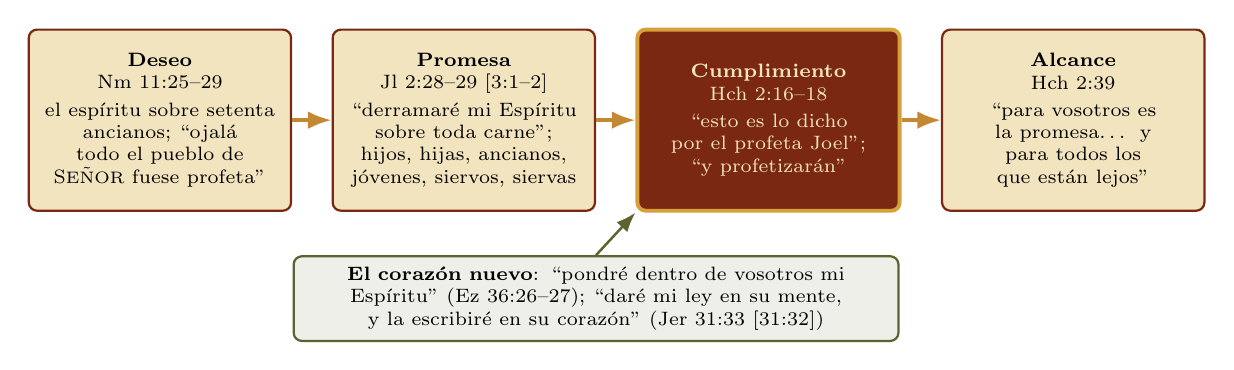
\begin{tikzpicture}[font=\scriptsize,node distance=0.5cm,
  bx/.style={draw=tierraroja,line width=0.8pt,fill=papiro,rounded corners=3pt,text width=3.05cm,align=center,inner sep=4pt,minimum height=2.3cm}]
 \node[bx] (n) {\textbf{Deseo}\\ Nm 11:25--29\\[2pt] el espíritu sobre setenta ancianos; ``ojalá todo el pueblo de \SENOR{} fuese profeta''};
 \node[bx,right=of n] (j) {\textbf{Promesa}\\ Jl 2:28--29 [3:1--2]\\[2pt] ``derramaré mi Espíritu sobre toda carne''; hijos, hijas, ancianos, jóvenes, siervos, siervas};
 \node[bx,right=of j,draw=mostaza,line width=1.4pt,fill=tierraroja,text=papiro] (h) {\textbf{Cumplimiento}\\ Hch 2:16--18\\[2pt] ``esto es lo dicho por el profeta Joel''; ``y profetizarán''};
 \node[bx,right=of h] (l) {\textbf{Alcance}\\ Hch 2:39\\[2pt] ``para vosotros es la promesa\ldots{} y para todos los que están lejos''};
 \foreach \u/\v in {n/j,j/h,h/l} \draw[-{Latex[length=3mm]},mostaza!80!tierraroja,line width=1.3pt] (\u)--(\v);
 \node[draw=oliva,line width=0.8pt,fill=oliva!10,rounded corners=3pt,text width=7.4cm,align=center,inner sep=4pt,below=0.55cm of j.south east] (e) {\textbf{El corazón nuevo}: ``pondré dentro de vosotros mi Espíritu'' (Ez 36:26--27); ``daré mi ley en su mente, y la escribiré en su corazón'' (Jer 31:33 [31:32])};
 \draw[-{Latex[length=2.5mm]},oliva,line width=0.9pt] (e.north) -- (h.south west);
\end{tikzpicture}}\par\medskip
\small\RaggedRight La lista de Joel recuerda Dt 16:11: en Shavuot se alegran ``tu hijo, tu hija, tu siervo, tu sierva''; en Joel reciben el Espíritu ``hijos e hijas\ldots{} siervos y siervas'' {\footnotesize\color{sepia}(observación propia)}.
\end{frame}

\begin{frame}{Babel invertida; la ley en el corazón}
\begin{columns}[t,onlytextwidth]
\begin{column}{0.48\textwidth}\small\RaggedRight
\textbf{Babel (Gn 11:7)}: ``confundamos allí su lengua'', LXX \grc{συγχέωμεν}. En Hch 2:6 la multitud ``estaba confusa'' (\grc{συνεχύθη}), con el mismo verbo en dirección contraria: allí la confusión dispersa, aquí \destacar{reúne}, y cada uno oye ``en su propia lengua''.\par\smallskip
\precision{eco señalado por Bruce (1988) y Keener (2012); Fitzmyer (1998) lo considera posible, no programático.}
\end{column}
\begin{column}{0.50\textwidth}
\begin{cita}\ldots{}escrita no con tinta, sino con el Espíritu del Dios vivo; no en tablas de piedra, sino en tablas de carne del corazón.\fuente{(2~Co 3:3)}\end{cita}
\scriptsize\RaggedRight ``Tablas de piedra'' = Sinaí (Éx 31:18); ``corazón de carne'' = Ez 36:26; ley en el corazón = Jer 31:33 (Hays, 1989). ``Las primicias del Espíritu'' (Ro 8:23).\par
\precision{Pablo no nombra Shavuot: el vínculo es temático.}
\end{column}
\end{columns}
\end{frame}

% ------------------------------------------------------------------
\section{La serie}

\begin{frame}{Memorial y figura}
\small\RaggedRight La fiesta de la Siega es memorial de \destacar{la manifestación del Espíritu de Dios en el monte Sinaí} y de la entrega de la Ley.\par\smallskip
\scriptsize\renewcommand{\arraystretch}{1.15}
\begin{tabular}{@{}L{3.0cm}L{2.3cm}L{6.6cm}@{}}
\toprule
\textbf{Hito de Israel} & \textbf{Fiesta} & \textbf{Nuevo Pacto (lectura de la serie)} \\ \midrule
Manifestación en el Sinaí y entrega de la Ley & Pentecostés, Siega, Semanas & Derramamiento del Espíritu (Hch 2); dos panes con levadura = pueblos aún con pecado considerados para la redención; lluvias de Joel 2:23 \\
\bottomrule
\end{tabular}\par\medskip
\small\RaggedRight Rasgos de la fiesta: instituida para conmemorar el día en que se dio la Ley, de \destacar{mandato perpetuo}, declarada \destacar{sábado santo}. Lv 23 es el \emph{Reglamento del Culto}, con tres períodos: Primogénitos, Israel, Iglesia.
\end{frame}

\begin{frame}{Dos precisiones al memorial}
\begin{columns}[t,onlytextwidth]
\begin{column}{0.49\textwidth}\small\RaggedRight
\textbf{Abraham en Mamre.} La serie ve una lengua de fuego, a semejanza de la manifestación de Pentecostés. El texto: ``un horno humeando, y una \destacar{antorcha de fuego}'' (Gn 15:17).\par\smallskip
\precision{\heb{לַפִּיד אֵשׁ} (\emph{lapid esh}) es la palabra de las ``antorchas'' del Sinaí (Éx 20:18): el vínculo Gn 15--Éx 20 es léxico, y el vínculo con Hch 2, tipológico.}
\end{column}
\begin{column}{0.49\textwidth}\small\RaggedRight
\textbf{¿``Sábado santo''?} Lv 23:21: \emph{mikrá kódesh} y ``ningún trabajo de siervos'' (\heb{מְלֶאכֶת עֲבֹדָה}).\par\smallskip
\precision{a diferencia de Teruá, Kipur y Sukkot (Lv 23:24, 32, 39), el texto no lo llama \emph{shabat} ni \emph{shabatón}: es reposo festivo y convocación, no sábado semanal.}\par\medskip
\textbf{La figura.} ¿Cómo pudo manifestarse el Espíritu sobre ellos si celebraban una fiesta presuntamente obsoleta? Cuarenta días de apariciones (Hch 1:3) + diez = el día cincuenta.
\end{column}
\end{columns}
\end{frame}

\begin{frame}{Los dos panes según la serie}
\small\RaggedRight La Congregación de los Primogénitos ya está alistada en los cielos (He 12:22--24). Falta todavía que se consume la salvación de Israel, lo que sucederá cuando se haya integrado al pueblo de Dios la plenitud de los gentiles. Estos \destacar{dos estamentos}, a pesar de su pecado, están considerados delante de Dios para su redención, y los representan los \destacar{dos panes con levadura}.\par\medskip
\small\RaggedRight \destacar{Levadura} = pecado aún presente; \destacar{primicias} = ya de Dios. Los ``dos estamentos'': por el antecedente más cercano, \textbf{Israel} y \textbf{la plenitud de los gentiles}; por la formulación completa, \textbf{la Congregación de los Primogénitos} e \textbf{Israel} (con los gentiles). Distintos del \emph{ómer} (Cristo) y de la Iglesia sin levadura (Ázimos).
\end{frame}

\begin{frame}{El \emph{ómer} y los dos panes}
\centering
\resizebox{\linewidth}{!}{%
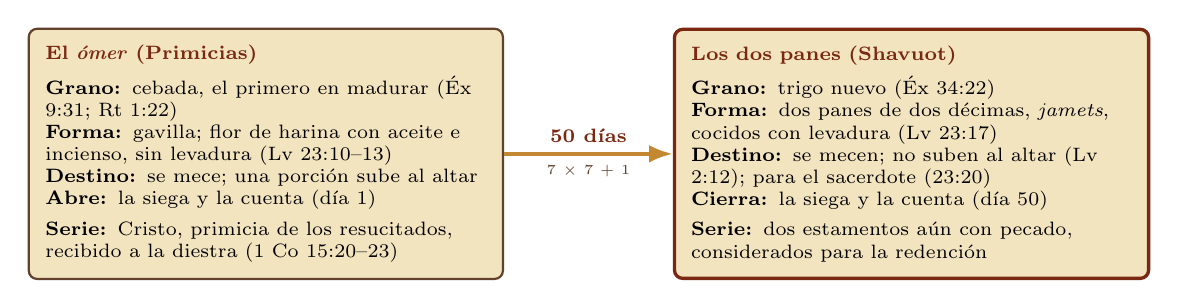
\begin{tikzpicture}[font=\scriptsize,
  co/.style={draw=sepia,line width=0.8pt,fill=papiro,rounded corners=3pt,text width=5.6cm,align=left,inner sep=6pt}]
 \node[co] (o) at (0,0) {\textbf{\color{tierraroja}El \emph{ómer} (Primicias)}\\[3pt]
  \textbf{Grano:} cebada, el primero en madurar (Éx 9:31; Rt 1:22)\\
  \textbf{Forma:} gavilla; flor de harina con aceite e incienso, sin levadura (Lv 23:10--13)\\
  \textbf{Destino:} se mece; una porción sube al altar\\
  \textbf{Abre:} la siega y la cuenta (día 1)\\[3pt]
  \textbf{Serie:} Cristo, primicia de los resucitados, recibido a la diestra (1~Co 15:20--23)};
 \node[co,draw=tierraroja,line width=1.2pt] (p) at (8.2,0) {\textbf{\color{tierraroja}Los dos panes (Shavuot)}\\[3pt]
  \textbf{Grano:} trigo nuevo (Éx 34:22)\\
  \textbf{Forma:} dos panes de dos décimas, \emph{jamets}, cocidos con levadura (Lv 23:17)\\
  \textbf{Destino:} se mecen; no suben al altar (Lv 2:12); para el sacerdote (23:20)\\
  \textbf{Cierra:} la siega y la cuenta (día 50)\\[3pt]
  \textbf{Serie:} dos estamentos aún con pecado, considerados para la redención};
 \draw[-{Latex[length=3mm]},mostaza!80!tierraroja,line width=1.4pt] (o.east) -- node[above,font=\scriptsize\bfseries,text=tierraroja]{50 días} node[below,font=\tiny,text=sepia]{7 $\times$ 7 + 1} (p.west);
\end{tikzpicture}}\par\medskip
\scriptsize\RaggedRight\precision{(1) La levadura no siempre es pecado: sí en 1 Co 5:6--8 y Gá 5:9; en Mt 13:33 (texto que la serie usa para las tres etapas) es el reino que crece. (2) La autoría de Hebreos es discutida (Attridge, 1989; Lane, 1991); el argumento descansa en el contenido de He 12:22--24. (3) Efesios (Ef 3:1--6) también es de autoría discutida; cf. Ro 11:17--26. (4) Levítico no explica los panes: la lectura es tipológica.}
\end{frame}

\begin{frame}{Las lluvias de Joel 2:23 según la serie}
\centering
\resizebox{!}{0.56\textheight}{%
\begin{tikzpicture}[font=\scriptsize,
  rb/.style={draw=oliva,line width=0.8pt,fill=oliva!10,rounded corners=3pt,text width=3.25cm,align=center,inner sep=4pt,minimum height=1.55cm},
  sb/.style={draw=tierraroja,line width=0.8pt,fill=papiro,rounded corners=3pt,text width=3.25cm,align=center,inner sep=4pt,minimum height=1.55cm}]
 \node[font=\scriptsize\bfseries,text=oliva!70!black,anchor=west] at (-1.9,1.25) {Jl 2:23 (orden del versículo)};
 \foreach \i/\h/\t/\f in {0/{\heb{הַמּוֹרֶה לִצְדָקָה}}/{``la primera lluvia arregladamente''}/{lluvia o maestro},1/{\heb{מוֹרֶה}}/{``lluvia temprana''}/{otoño: \emph{yoré}},2/{\heb{מַלְקוֹשׁ}}/{``tardía''}/{primavera},3/{\heb{בָּרִאשׁוֹן}}/{``como al principio''}/{adverbio: ``en el primero''}}{
   \node[rb] (r\i) at (\i*3.85,0) {\large\h\\[1pt] \scriptsize\t\\ {\tiny\color{sepia}\f}};}
 \foreach \i/\s in {0/{El Espíritu en algunos de Israel: sacerdotes, profetas, reyes; no siempre ni en todos},1/{El Aposento Alto (Hch 2), extendido a la Iglesia del Nuevo Pacto},2/{Israel en el tiempo del fin, cuando entre el último de los gentiles},3/{La Congregación de los Primogénitos: Dios cara a cara}}{
   \node[sb] (s\i) at (\i*3.85,-2.15) {\s};
   \draw[-{Latex[length=2mm]},sepia,line width=0.7pt] (r\i.south) -- (s\i.north);}
 \node[font=\scriptsize\bfseries,text=tierraroja,anchor=west] at (-1.9,-3.65) {Orden histórico según la serie};
 \draw[line width=1.4pt,tierraroja,-{Latex[length=3mm]}] (-1.7,-4.7) -- (13.4,-4.7);
 \foreach \x/\t/\c in {-0.6/{1. Primogénitos}/{``del principio''},3.3/{2. Israel}/{``la primera, arregladamente''},7.2/{3. Iglesia}/{``temprana''},11.1/{4. Israel al fin}/{``tardía''}}{
   \fill[mostaza] (\x+0.6,-4.7) circle (3.5pt);
   \node[above=4pt,font=\scriptsize\bfseries,text=caferojizo] at (\x+0.6,-4.7) {\t};
   \node[below=4pt,font=\tiny,text=sepia] at (\x+0.6,-4.7) {\c};}
\end{tikzpicture}}\par\smallskip
\scriptsize\RaggedRight Apoyo textual: Joel pasa de la lluvia (2:23) al Espíritu derramado (\heb{אֶשְׁפּוֹךְ}, 3:1) ``después de esto''; cf. Is 44:3; Os 6:3.\par
\precision{en hebreo hay \textbf{dos} lluvias (\emph{moré} = \emph{yoré}, otoño; \emph{malqosh}, primavera), un \emph{hamoré} discutido (lluvia o maestro) y un adverbio (\emph{barishón}). La serie usa ``temprana/tardía'' como secuencia histórica, no como estación (Shavuot cae en la estación seca); las identificaciones son suyas; cf. otra lectura de la ``lluvia tardía'' en Myland (1910).}
\end{frame}

\begin{frame}{Shavuot y el pacto matrimonial}
\begin{columns}[t,onlytextwidth]
\begin{column}{0.50\textwidth}\small\RaggedRight
Figura que desarrollé en mi presentación anterior: Shavuot como \destacar{boda del Mesías (novio) con Israel (novia)}, en dos etapas:
\begin{itemize}
\item \textbf{Compromiso} (\emph{erusín}): contrato; legalmente casados, sin cohabitar.
\item \textbf{Boda} (\emph{nisuín}): el novio lleva a la novia a su casa.
\end{itemize}
Éx 19--24 tiene la forma del pacto: propuesta (19:5--6), consentimiento (``haremos'', 19:8; 24:3, 7), documento (24:4) y comida ante Dios (24:11).
\end{column}
\begin{column}{0.48\textwidth}\scriptsize\RaggedRight
\begin{cita}\ldots{}porque ellos invalidaron mi pacto, aunque fui yo un marido para ellos, dice \SENOR.\fuente{(Jer 31:32)}\end{cita}
``El amor de tu desposorio\ldots{} en el desierto'' (Jer 2:2); ``te desposaré conmigo para siempre'' (Os 2:19--20); Cristo y la iglesia (Ef 5:25--32; 2 Co 11:2); ``las bodas del Cordero'' (Ap 19:7--9). La Misná: ``el día de su desposorio'' (Cnt 3:11) = la entrega de la Torá (m. Taanit 4:8).\par\smallskip
\precision{lectura tipológica: ningún texto llama a Shavuot ``compromiso''; las etapas \emph{erusín}/\emph{nisuín} son de la ley rabínica.}
\end{column}
\end{columns}
\end{frame}

\begin{frame}{Las arras del Espíritu}
\begin{columns}[c,onlytextwidth]
\begin{column}{0.52\textwidth}
\begin{cita}El cual también nos ha sellado, y nos ha dado las arras del Espíritu en nuestros corazones.\fuente{(2~Co 1:22)}\end{cita}
\begin{cita}\ldots{}fuisteis sellados con el Espíritu Santo de la promesa, que es las arras de nuestra herencia\ldots\fuente{(Ef 1:13--14)}\end{cita}
\end{column}
\begin{column}{0.46\textwidth}\small\RaggedRight
\grc{ἀρραβών} (\emph{arrabōn}, G728): \destacar{pago adelantado} que garantizaba una compra; se perdía si la compra no se efectuaba.\par\smallskip
Préstamo semítico: \heb{עֵרָבוֹן} (\emph{eravón}), la prenda de Judá a Tamar (Gn 38:17--18, 20; LXX \grc{ἀρραβών}).\par\smallskip
En griego moderno, \emph{arrabōna} significa compromiso y anillo de compromiso. Junto a Ro 8:23 (``las primicias del Espíritu''), el Espíritu es \destacar{primicia y prenda}, y la cosecha y la boda vienen después.\par\smallskip\scriptsize ``Si las primicias son santas, también lo es la masa'' (Ro 11:16); ``lluvia temprana y tardía'' (Stg 5:7); ``primicias para Dios y para el Cordero'' (Ap 14:4).
\end{column}
\end{columns}
\end{frame}

\begin{frame}{Pentecostés en la Iglesia apostólica}
\begin{columns}[c,onlytextwidth]
\begin{column}{0.52\textwidth}
\begin{cita}\ldots{}pues se apresuraba por estar el día de Pentecostés, si le fuese posible, en Jerusalén.\fuente{(Hch 20:16)}\end{cita}
\begin{cita}Pero estaré en Éfeso hasta Pentecostés.\fuente{(1~Co 16:8)}\end{cita}
\end{column}
\begin{column}{0.46\textwidth}\small\RaggedRight
La serie: también esa \destacar{iglesia gentil} guardaba la fiesta.\par\medskip
\precision{Hch 20:16 es un viaje de peregrinación. 1 Co 16:8 admite dos lecturas: observancia en Éfeso (la serie) o referencia de calendario (Fee, 1987). Ningún texto describe cómo la celebraba una iglesia gentil.}
\end{column}
\end{columns}
\end{frame}

% ------------------------------------------------------------------
\section{Mesías}

\begin{frame}{La promesa del Padre y la siega}
\begin{columns}[t,onlytextwidth]
\begin{column}{0.49\textwidth}\small\RaggedRight
\begin{itemize}
\item ``Quedaos\ldots{} hasta que seáis investidos de poder desde lo alto'' (Lc 24:49); ``la promesa del Padre'' (Hch 1:4--5).
\item Cuarenta días de apariciones (Hch 1:3); el Espíritu llega ``al cumplirse'' el día cincuenta.
\item Pedro: el exaltado ``ha derramado esto que vosotros veis y oís'' (Hch 2:33).
\item Jn 20:22, ``Recibid el Espíritu Santo'': ¿anticipo o versión joánica? Se discute.
\end{itemize}
\end{column}
\begin{column}{0.49\textwidth}\small\RaggedRight
\begin{itemize}
\item ``La mies es mucha, mas los obreros pocos'' (Mt 9:37--38); ``los campos\ldots{} blancos para la siega'' (Jn 4:35): \grc{θερισμός}, el griego de \emph{qatsir}.
\item Tres mil en un día, la primera siega abundante (Hch 2:41).
\end{itemize}
\precision{Baker (2013) une Lv 23:22 con Mt 12:1; la ley de esa escena es Dt 23:25 [23:26], y el debate es sobre el sábado.}
\end{column}
\end{columns}
\end{frame}

% ------------------------------------------------------------------
\section{Tradición}

\begin{frame}{Shavuot en la tradición judía}
\begin{columns}[t,onlytextwidth]
\begin{column}{0.49\textwidth}\small\RaggedRight
\begin{itemize}
\item \heb{עֲצֶרֶת} \emph{Atséret}: ``clausura'' de Pésaj (m. Rosh Hashaná 1:2; Josefo).
\item Procesión de \emph{bikurim} con flauta y buey adornado (m. Bikurim 3:2--4); no antes de Atséret (1:3).
\item Panes de siete por cuatro palmos, con ``cuernos'' (m. Menajot 11:4).
\item ``El día en que fue dada la Torá'' (b. Pesajim 68b); lecturas: Dt 16:9 y Hab 3, o Éx 19 y Ez 1 (b. Meguilá 31a).
\end{itemize}
\end{column}
\begin{column}{0.49\textwidth}
\begin{tcolorbox}[colback=mostaza!10,colframe=mostaza!85!tierraroja,boxrule=0.6pt,arc=2pt,left=4pt,right=4pt,fonttitle=\bfseries\scriptsize,coltitle=caferojizo,colbacktitle=mostaza!30,title={Precisión: prácticas posteriores}]
\scriptsize\RaggedRight Cada palabra del Sinaí se dividió en setenta lenguas (b. Shabbat 88b), tradición varios siglos posterior a Hechos. También son posteriores \emph{sefirat haómer} con bendición, la lectura de Rut (\emph{Soferim} 14:3), \emph{Akdamut} (s.~\textsc{xi}), \emph{tikún leil Shavuot} (Safed, s.~\textsc{xvi}) y los lácteos y las ramas verdes. Ninguna figura en la Torá.
\end{tcolorbox}
\end{column}
\end{columns}
\end{frame}

\begin{frame}{Las tres trompetas}
\begin{columns}[c,onlytextwidth]
\begin{column}{0.60\textwidth}
\resizebox{\linewidth}{!}{%
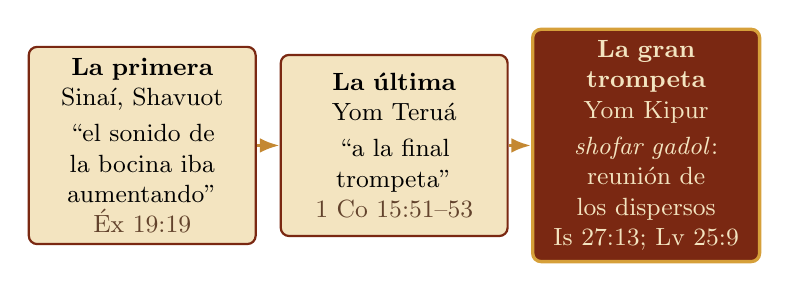
\begin{tikzpicture}[font=\small,
  tr/.style={draw=tierraroja,line width=0.8pt,fill=papiro,rounded corners=3pt,text width=2.6cm,align=center,inner sep=4pt,minimum height=2.3cm}]
 \node[tr] (a) at (0,0) {\textbf{La primera}\\ Sinaí, Shavuot\\[2pt] ``el sonido de la bocina iba aumentando'' \\ {\color{sepia}Éx 19:19}};
 \node[tr] (b) at (3.2,0) {\textbf{La última}\\ Yom Teruá\\[2pt] ``a la final trompeta'' \\ {\color{sepia}1 Co 15:51--53}};
 \node[tr,fill=tierraroja,text=papiro,draw=mostaza,line width=1.2pt] (c) at (6.4,0) {\textbf{La gran trompeta}\\ Yom Kipur\\[2pt] \emph{shofar gadol}: reunión de los dispersos \\ {\color{papiro}Is 27:13; Lv 25:9}};
 \draw[-{Latex[length=2.5mm]},mostaza!80!tierraroja,line width=1.2pt] (a)--(b);
 \draw[-{Latex[length=2.5mm]},mostaza!80!tierraroja,line width=1.2pt] (b)--(c);
\end{tikzpicture}}
\end{column}
\begin{column}{0.38\textwidth}\small\RaggedRight
Asociación judía que recogí en mi presentación anterior. Un \emph{midrash}: de los cuernos del carnero de Isaac, uno sonó en el Sinaí y el otro sonará en Is 27:13 (\emph{Pirké de Rabí Eliezer} 31).\par\medskip
\precision{los textos son bíblicos; su orden como primera, última y gran trompeta y su asignación a las fiestas son tradición y tipología.}
\end{column}
\end{columns}
\end{frame}

% ------------------------------------------------------------------
\section{Discusión}

\begin{frame}{Dos debates abiertos}
\begin{columns}[t,onlytextwidth]
\begin{column}{0.49\textwidth}
\begin{tcolorbox}[colback=papiro,colframe=sepia,boxrule=0.7pt,arc=2pt,left=4pt,right=4pt,fonttitle=\bfseries\scriptsize,coltitle=papiro,colbacktitle=sepia,title={¿Fiesta agrícola o del pacto?}]
\scriptsize\RaggedRight \textbf{Agrícola en su origen}, con el Sinaí como relectura posterior (de Vaux, 1985).\\ \textbf{Pacto desde antiguo}: Éx 19:1; 2 Cr 15; Jubileos; Qumrán (Weinfeld, 1978; VanderKam, 1998).\\ Las posiciones no se excluyen, pues la siega es también memoria del siervo liberado (Dt 16:12).
\end{tcolorbox}
\end{column}
\begin{column}{0.49\textwidth}
\begin{tcolorbox}[colback=papiro,colframe=tierraroja,boxrule=0.7pt,arc=2pt,left=4pt,right=4pt,fonttitle=\bfseries\scriptsize,coltitle=papiro,colbacktitle=tierraroja,title={¿Lucas narra con el Sinaí al fondo?}]
\scriptsize\RaggedRight \textbf{Sí}: Kretschmar (1954), Dunn (1970), Turner (1996); con matices, Bruce (1988), Keener (2012); cf. Sal 68:18 y Ef 4:8.\\ \textbf{Con cautela}: Haenchen (1971), Fitzmyer (1998), para quienes el texto se explica por Joel y la misión.\\ La lectura canónica no depende de la intención de Lucas.
\end{tcolorbox}
\end{column}
\end{columns}
\end{frame}

\begin{frame}{Los dos panes: lecturas}
\scriptsize\renewcommand{\arraystretch}{1.18}
\begin{tabular}{@{}L{2.9cm}L{5.4cm}L{3.6cm}@{}}
\toprule
\textbf{Lectura} & \textbf{Levadura y número dos} & \textbf{Autores} \\ \midrule
Dos estamentos aún con pecado & pecado aún presente; dos pueblos considerados para la redención & Lectura de la serie \\
Judíos y gentiles en un pueblo & humanidad pecadora redimida; la Iglesia de judíos y gentiles (Ef 2:14--16) & Chumney (1994); Howard y Rosenthal (1997); Baker (2013) \\
La Iglesia con mal aún presente & el mal que persiste en los redimidos, aceptados por el sacrificio & Mackintosh (1861) \\
Histórico-sacerdotal & pan ordinario de la casa: la siega como alimento; por eso no va al altar & Milgrom (2001); Hartley (1992); Wenham (1979) \\
\bottomrule
\end{tabular}\par\medskip
\small\RaggedRight Las tres primeras coinciden en que las primicias \destacar{con levadura} son de Dios sin estar libres de toda imperfección; difieren en quiénes son los dos.
\end{frame}

% ------------------------------------------------------------------
\section{Síntesis}

\begin{frame}{Shavuot: definición}
\begin{tcolorbox}[colback=papiro,colframe=tierraroja,boxrule=1pt,arc=3pt]
\small\RaggedRight Fiesta de la siega del trigo a la que Israel llega \destacar{contando} siete semanas cumplidas desde el \emph{ómer} (Lv 23:15--16). Se presenta una \destacar{ofrenda nueva}: dos panes leudados, mecidos y no quemados (23:17; 2:12), y se deja el borde del campo al pobre y al extranjero (23:22). Es fiesta de \destacar{alegría inclusiva} y de \destacar{memoria} del siervo (Dt 16:11--12). El Segundo Templo la leyó como \destacar{fiesta del pacto} (Éx 19:1), y en ella Dios derramó su \destacar{Espíritu} (Hch 2): la ley en tablas de carne (2 Co 3:3), las primicias del Espíritu (Ro 8:23).
\end{tcolorbox}
\scriptsize\renewcommand{\arraystretch}{1.08}
\begin{tabular}{@{}L{1.8cm}L{10.1cm}@{}}
\toprule
Histórica & siega del trigo en la estación seca; Rut; peregrinación; diáspora reunida; Sinaí en Jubileos y Qumrán \\
Filológica & \emph{shavuot}/\emph{shevuá}; \emph{temimot}; \emph{jamets} y Lv 2:12; \emph{peá}, \emph{léqet}; \emph{qolot}, \emph{lapidim}; lenguas de fuego; \emph{yoré}, \emph{malqosh}, \emph{moré} \\
Textual & cómputo de Lv 23:15--16; Jl 2:23 TM/LXX/Vulgata; Hch 2:17 \\
Literaria & Lv 23:9--22; Sinaí--Hch 2; Nm 11 $\rightarrow$ Jl 3 $\rightarrow$ Hch 2; Babel; Jer 31; 2 Co 3 \\
La serie & memorial del Sinaí; figura del Espíritu; dos panes; cuatro lluvias; fiesta guardada \\
\bottomrule
\end{tabular}
\end{frame}

% ------------------------------------------------------------------
\section{Reflexión}

\begin{frame}{Para la reflexión}
\small
\begin{enumerate}
\item ¿Qué cambia en la espera cuando se cuenta día por día, como entre la primicia y la cosecha (Lv 23:15--16; Hch 1:3--5)?
\item Los panes vienen ``de vuestras habitaciones'' y llevan levadura. ¿Qué implica presentar a Dios el pan ordinario de la casa?
\item Si la alegría de Shavuot incluía al siervo, al extranjero, al huérfano y a la viuda (Dt 16:11), ¿a quién deja fuera hoy nuestra alegría? ¿Qué ``rincón del campo'' nos toca dejar?
\item ¿Dónde se nota, en concreto, la diferencia entre una ley escrita en piedra y una escrita en el corazón (2 Co 3:3)?
\item ¿A quiénes se trata en la comunidad como si no hubieran recibido el Espíritu (Nm 11:29; Jl 2:29)?
\end{enumerate}
\end{frame}

% ------------------------------------------------------------------
\section{Glosario}

\begin{frame}{Glosario}
\scriptsize
\begin{columns}[t,onlytextwidth]
\begin{column}{0.49\textwidth}\RaggedRight
\textbf{\emph{Atséret}} (\heb{עֲצֶרֶת}): ``clausura''; nombre rabínico de Shavuot.\par\smallskip
\textbf{\emph{Bikurim}} (\heb{בִּכּוּרִים}): primicias.\par\smallskip
\textbf{\emph{Jag}} (\heb{חַג}): fiesta de peregrinación.\par\smallskip
\textbf{\emph{Jamets}} (\heb{חָמֵץ}): lo leudado.\par\smallskip
\textbf{\emph{Léqet}} (\heb{לֶקֶט}): espigueo para el pobre.\par\smallskip
\textbf{\emph{Malqosh}} (\heb{מַלְקוֹשׁ}): lluvia tardía de primavera.\par\smallskip
\textbf{\emph{Minjá jadashá}} (\heb{מִנְחָה חֲדָשָׁה}): ofrenda nueva.\par\smallskip
\textbf{\emph{Moré}} (\heb{מוֹרֶה}): lluvia temprana; ``maestro''.
\end{column}
\begin{column}{0.49\textwidth}\RaggedRight
\textbf{\emph{Peá}} (\heb{פֵּאָה}): rincón del campo.\par\smallskip
\textbf{Pentecostés} (\grc{πεντηκοστή}): ``el quincuagésimo''.\par\smallskip
\textbf{\emph{Qolot}} (\heb{קֹלֹת}): ``voces'', truenos del Sinaí.\par\smallskip
\textbf{\emph{Shavuot}} (\heb{שָׁבֻעוֹת}): semanas.\par\smallskip
\textbf{\emph{Shevuá}} (\heb{שְׁבוּעָה}): juramento.\par\smallskip
\textbf{\emph{Temimot}} (\heb{תְּמִימֹת}): cumplidas, completas.\par\smallskip
\textbf{\emph{Tenufá}} (\heb{תְּנוּפָה}): ofrenda mecida.\par\smallskip
\textbf{\emph{Yoré}} (\heb{יוֹרֶה}): lluvia temprana de otoño.
\end{column}
\end{columns}
\end{frame}

% ------------------------------------------------------------------
\section{Referencias}

\begin{frame}{Referencias}
\fontsize{4.8}{5.6}\selectfont
\textit{Citas bíblicas: Reina-Valera 1960, con \SENOR{} donde dice ``Jehová''; hebreo BHS; griego NA28 y Rahlfs-Hanhart. Tobías y 2 Macabeos: fuentes históricas deuterocanónicas.}\par\smallskip
\begin{columns}[t,onlytextwidth]
\begin{column}{0.49\textwidth}
\refapa{Ahlström, G.~W. (1971). \emph{Joel and the temple cult of Jerusalem}. Brill.}
\refapa{Attridge, H.~W. (1989). \emph{The epistle to the Hebrews}. Fortress.}
\refapa{Baker, D. (2013). \emph{El poder espiritual de las siete fiestas de Dios}. Editorial Imagen.}
\refapa{Borowski, O. (1987). \emph{Agriculture in Iron Age Israel}. Eisenbrauns.}
\refapa{Bruce, F.~F. (1988). \emph{The book of the Acts} (ed. rev.). Eerdmans.}
\refapa{Chumney, E. (1994). \emph{The seven festivals of the Messiah}. Destiny Image.}
\refapa{Crenshaw, J.~L. (1995). \emph{Joel} (AB 24C). Doubleday.}
\refapa{de Vaux, R. (1985). \emph{Instituciones del Antiguo Testamento}. Herder.}
\refapa{Dunn, J.~D.~G. (1970). \emph{Baptism in the Holy Spirit}. SCM.}
\refapa{Elliger, K., \& Rudolph, W. (Eds.). (1997). \emph{Biblia Hebraica Stuttgartensia} (5.ª ed.). Deutsche Bibelgesellschaft.}
\refapa{Fee, G.~D. (1987). \emph{The first epistle to the Corinthians}. Eerdmans.}
\refapa{Filón de Alejandría. (1937). \emph{De Decalogo} (F.~H. Colson, Trad.; Loeb 7). Harvard University Press.}
\refapa{Fitzmyer, J.~A. (1998). \emph{The Acts of the Apostles} (AB 31). Doubleday.}
\refapa{Flavio Josefo. (1997). \emph{Antigüedades judías} (J. Vara Donado, Trad.). Akal.}
\refapa{Flavio Josefo. (1997). \emph{La guerra de los judíos I--III} (J.~M. Nieto Ibáñez, Trad.). Gredos.}
\refapa{Gómez Correa, D. (s.\,f.). \emph{Pentecostés} [Presentación, proyecto «Fiestas Santas»].}
\refapa{Haenchen, E. (1971). \emph{The Acts of the Apostles}. Westminster.}
\refapa{Hartley, J.~E. (1992). \emph{Leviticus} (WBC 4). Word.}
\refapa{Hays, R.~B. (1989). \emph{Echoes of Scripture in the letters of Paul}. Yale University Press.}
\refapa{Howard, K., \& Rosenthal, M. (1997). \emph{The feasts of the Lord}. Thomas Nelson.}
\end{column}
\begin{column}{0.49\textwidth}
\refapa{Keener, C.~S. (2012). \emph{Acts: An exegetical commentary} (Vol. 1). Baker Academic.}
\refapa{Kretschmar, G. (1954). Himmelfahrt und Pfingsten. \emph{Zeitschrift für Kirchengeschichte, 66}, 209--253.}
\refapa{Lane, W.~L. (1991). \emph{Hebrews} (WBC 47A--B). Word.}
\refapa{Mackintosh, C.~H. (1861). \emph{Notes on the book of Leviticus}. G. Morrish.}
\refapa{Milgrom, J. (1991). \emph{Leviticus 1--16} (AB 3). Doubleday.}
\refapa{Milgrom, J. (2001). \emph{Leviticus 23--27} (AB 3B). Doubleday.}
\refapa{Myland, D.~W. (1910). \emph{The latter rain covenant and Pentecostal power}. Evangel.}
\refapa{Nestle, E., \& Aland, K. (Eds.). (2012). \emph{Novum Testamentum Graece} (28.ª ed.). Deutsche Bibelgesellschaft.}
\refapa{Rahlfs, A., \& Hanhart, R. (Eds.). (2006). \emph{Septuaginta} (ed. rev.). Deutsche Bibelgesellschaft.}
\refapa{Scott, J.~M. (1994). Luke's geographical horizon. En D.~W.~J. Gill \& C. Gempf (Eds.), \emph{The book of Acts in its Graeco-Roman setting} (pp. 483--544). Eerdmans.}
\refapa{Sefaria. (s.\,f.). \emph{Talmud Bavli; Midrash Rabbah; Masekhet Soferim}. https://www.sefaria.org}
\refapa{Sociedades Bíblicas en América Latina. (1960). \emph{Santa Biblia: Reina-Valera 1960}.}
\refapa{Turner, M. (1996). \emph{Power from on high}. Sheffield Academic Press.}
\refapa{VanderKam, J.~C. (1998). \emph{Calendars in the Dead Sea Scrolls}. Routledge.}
\refapa{VanderKam, J.~C. (2001). \emph{The book of Jubilees}. Sheffield Academic Press.}
\refapa{Weinfeld, M. (1978). Pentecost as festival of the giving of the Law. \emph{Immanuel, 8}, 7--18.}
\refapa{Wenham, G.~J. (1979). \emph{The book of Leviticus} (NICOT). Eerdmans.}
\refapa{Wolff, H.~W. (1977). \emph{Joel and Amos} (Hermeneia). Fortress.}
\end{column}
\end{columns}
\end{frame}

\end{document}
